%!TEX TS-program = pdflatex
%!TEX TS-options = -shell-escape
% ============================================================
%  Prinzipien der Robotik
%  Vorlesung Embedded Systems Engineering
%  Prof. Dr.-Ing. Sebastian Schlesinger
%  HWR Berlin, Wintersemester 2026
% ============================================================

% xcolor muss vor beamer mit Optionen gepatcht werden
\PassOptionsToPackage{usenames,x11names}{xcolor}

\documentclass[%
  aspectratio=169,
  10pt
]{beamer}

% -----------------------------------------------------------
%  Sprache und Encoding
% -----------------------------------------------------------
\usepackage[utf8]{inputenc}
\usepackage[T1]{fontenc}
\usepackage{textcomp}
\newcommand{\enquote}[1]{\quotedblbase{}#1\textquotedblleft{}}

% -----------------------------------------------------------
%  Fonts
% -----------------------------------------------------------
\usepackage{charter}
\usepackage{courier}
\renewcommand{\ttdefault}{pcr}
\usepackage[protrusion=true,expansion=false]{microtype}

% -----------------------------------------------------------
%  Farben  (wie config.tex der Übungsblätter)
% -----------------------------------------------------------
\definecolor{fbblau}{HTML}{3078AB}
\definecolor{blackberry}{rgb}{0.53, 0.0, 0.25}
\definecolor{codebg}{rgb}{0.97, 0.97, 0.97}
\definecolor{dkgreen}{rgb}{0.0, 0.5, 0.0}

% -----------------------------------------------------------
%  Beamer-Theme (angepasst an ESE-Stil)
% -----------------------------------------------------------
\usetheme{default}
\useinnertheme{rectangles}

%  Strukturfarbe
\setbeamercolor{structure}{fg=fbblau}

%  Titelfolie
\setbeamercolor{title}{fg=white, bg=fbblau}
\setbeamercolor{subtitle}{fg=fbblau!25!white, bg=fbblau}
\setbeamercolor{author}{fg=white, bg=fbblau}
\setbeamercolor{institute}{fg=fbblau!20!white, bg=fbblau}
\setbeamercolor{date}{fg=fbblau!20!white, bg=fbblau}

%  Folienrahmen
\setbeamercolor{frametitle}{fg=white, bg=fbblau}
\setbeamerfont{frametitle}{series=\bfseries, size=\normalsize}

%  Inhaltsverzeichnis
\setbeamercolor{section in toc}{fg=fbblau}
\setbeamerfont{section in toc}{series=\bfseries}

%  Blöcke
\setbeamercolor{block title}{bg=fbblau, fg=white}
\setbeamercolor{block body}{bg=fbblau!8, fg=black}
\setbeamercolor{alertblock title}{bg=blackberry, fg=white}
\setbeamercolor{alertblock body}{bg=blackberry!8, fg=black}
\setbeamercolor{exampleblock title}{bg=fbblau!70!black, fg=white}
\setbeamercolor{exampleblock body}{bg=fbblau!6, fg=black}

%  Aufzählungspunkte
\setbeamercolor{item}{fg=fbblau}
\setbeamercolor{subitem}{fg=fbblau!70}
\setbeamertemplate{itemize item}{\small$\triangleright$}
\setbeamertemplate{itemize subitem}{\small$\triangleright$}

%  Navigationsleiste ausblenden
\setbeamertemplate{navigation symbols}{}

%  Fußzeile
\setbeamertemplate{footline}{%
  \leavevmode
  \hbox{%
    \begin{beamercolorbox}[wd=.50\paperwidth,ht=2.25ex,dp=1ex,
                           left,leftskip=2mm]{palette primary}%
      \usebeamerfont{author in head/foot}%
      \textbf{ESE} \,|\, Prinzipien der Robotik \,|\, \insertshortauthor
    \end{beamercolorbox}%
    \begin{beamercolorbox}[wd=.40\paperwidth,ht=2.25ex,dp=1ex,
                           center]{palette secondary}%
      \usebeamerfont{title in head/foot}\insertsection
    \end{beamercolorbox}%
    \begin{beamercolorbox}[wd=.10\paperwidth,ht=2.25ex,dp=1ex,
                           right,rightskip=2mm]{palette primary}%
      \insertframenumber\,/\,\inserttotalframenumber
    \end{beamercolorbox}%
  }%
}

%  Sectiontrenner
\AtBeginSection[]{%
  \begin{frame}[plain]
    \vfill
    \centering
    \begin{beamercolorbox}[sep=12pt,center,shadow=false,rounded=false,
                           wd=0.8\textwidth]{title}
      \usebeamerfont{title}\insertsectionhead
    \end{beamercolorbox}
    \vfill
  \end{frame}
}

% -----------------------------------------------------------
%  Code-Listings
% -----------------------------------------------------------
\usepackage{listings}
\lstset{%
  language        = C,
  basicstyle      = \ttfamily\footnotesize,
  keywordstyle    = \color{fbblau}\bfseries,
  commentstyle    = \color{gray}\itshape,
  stringstyle     = \color{blackberry},
  numberstyle     = \tiny\color{gray},
  numbers         = left,
  numbersep       = 8pt,
  stepnumber      = 1,
  frame           = single,
  framesep        = 3pt,
  rulecolor       = \color{fbblau!40},
  backgroundcolor = \color{codebg},
  showstringspaces= false,
  breaklines      = true,
  columns         = fullflexible,
  keepspaces      = true,
  xleftmargin     = 1.2em,
  xrightmargin    = 0.3em,
  tabsize         = 4,
  morekeywords    = {uint8_t,uint16_t,uint32_t,uint64_t,
                     int8_t,int16_t,int32_t,int64_t,
                     bool,true,false,NULL,size_t,
                     volatile,inline,restrict},
  literate        = {ä}{{\"a}}1 {ö}{{\"o}}1 {ü}{{\"u}}1
                    {Ä}{{\"A}}1 {Ö}{{\"O}}1 {Ü}{{\"U}}1
                    {ß}{{\ss}}1
}

\lstdefinelanguage{Python}{
  keywords={def,return,if,elif,else,for,while,import,from,as,class,
            self,True,False,None,with,lambda,try,except,raise,pass,
            and,or,not,in,is,print,range,len,np,float,int},
  keywordstyle=\color{fbblau}\bfseries,
  commentstyle=\color{gray}\itshape,
  stringstyle=\color{blackberry},
  morecomment=[l]{\#},
  morestring=[b]",
  morestring=[b]',
  sensitive=true
}

% -----------------------------------------------------------
%  Weitere Pakete
% -----------------------------------------------------------
\usepackage{tikz}
\usetikzlibrary{arrows.meta, shapes, positioning, calc, matrix,
                 decorations.pathreplacing, backgrounds, fit, decorations}
\usepgflibrary{decorations.pathreplacing}
\usepackage{booktabs}
\usepackage{array}
\usepackage{multicol}
\usepackage{amsmath,amssymb}
\usepackage{mathtools}
\usepackage{bm}
% SI-Einheiten (Fallback ohne siunitx)
\newcommand{\SI}[2]{#1\,\text{#2}}
\newcommand{\si}[1]{\text{#1}}

% -----------------------------------------------------------
%  Eigene Kommandos
% -----------------------------------------------------------
\newcommand{\hl}[1]{{\color{fbblau}\textbf{#1}}}
\newcommand{\warn}[1]{{\color{blackberry}\textbf{#1}}}
\newcommand{\R}{\mathbb{R}}

% -----------------------------------------------------------
%  Metadaten
% -----------------------------------------------------------
\title[Prinzipien der Robotik]{Prinzipien der Robotik}
\subtitle{Embedded Systems Engineering -- Vorlesung}
\author[Schlesinger]{Prof.\,Dr.\,-Ing.\ Sebastian Schlesinger}
\institute{%
  Fachbereich 2 -- Duales Studium Wirtschaft \& Technik\\
  HWR Berlin}
\date{Wintersemester 2026}

% ============================================================
\begin{document}
% ============================================================

% -----------------------------------------------------------
%  TITELFOLIE
% -----------------------------------------------------------
\begin{frame}[plain]
  \titlepage
\end{frame}

% -----------------------------------------------------------
%  GLIEDERUNG
% -----------------------------------------------------------
\begin{frame}{Gliederung}
  \tableofcontents
\end{frame}


% -----------------------------------------------------------
%  MOTIVATION: Brücke von Modellierung zu Robotik
% -----------------------------------------------------------
\begin{frame}{Von der Modellierung zur Implementierung}

\textbf{Bisherige Vorlesung:} Werkzeuge und Methoden der Modellierung
\begin{itemize}
  \item Software Engineering, FSMs, State Charts
  \item Timed Automata, Verifikation mit UPPAAL
  \item Programmierung in C und Rust
  \item ROS\,2 als Middleware
\end{itemize}

\pause
\vspace{3mm}
\textbf{Jetzt:} Wie setzt man diese Werkzeuge ein, um einen
\hl{realen Roboter} zu bauen und zu steuern?

\pause
\vspace{3mm}
\begin{alertblock}{Kernfrage}
  Wie kommt ein mobiler Roboter von Sensordaten zu sicherer,
  zielgerichteter Bewegung -- und wie verifizieren wir das?
\end{alertblock}
\end{frame}


% ============================================================
\section{Sensorsignale verstehen}
% ============================================================

% -----------------------------------------------------------
\begin{frame}{Sensormodelle -- Überblick}

Ein Roboter nimmt die Welt ausschließlich über \hl{Sensoren} wahr.
Jeder Sensor liefert ein \emph{Modell} der physikalischen Größe.

\vspace{3mm}
\begin{columns}[T]
  \begin{column}{0.48\textwidth}
    \textbf{Inertialsensoren (IMU)}
    \begin{itemize}
      \item Beschleunigungssensor: $a = F/m$
      \item Gyroskop: Winkelgeschwindigkeit $\omega$
      \item 6-DOF (degrees of freedom): $[a_x, a_y, a_z, \omega_x, \omega_y, \omega_z]^T$
    \end{itemize}
    $a_i$ ist die Beschleunigung entlang der $i$-ten Achse (Bewegung im Raum), $\omega_i$ die Winkelgeschwindigkeit um die $i$-te Achse (Drehung im Raum).
  \end{column}
  \begin{column}{0.48\textwidth}
    \textbf{Entfernungssensoren}
    \begin{itemize}
      \item Lidar / Ultraschall: Time-of-Flight
      \item $d = \frac{c \cdot \Delta t}{2}$
      \item Lidar: Laserpulse, $360°$-Scan
      \item Ultraschall: Schallkegel, geringere Auflösung
    \end{itemize}
  \end{column}
\end{columns}

\end{frame}


% -----------------------------------------------------------
\begin{frame}{Sensormodell: Kamera -- Projektionsmodell}

\begin{columns}[T]
  \begin{column}{0.55\textwidth}
    \textbf{Pinhole-Kameramodell:}
    $(u, v, w) = K \cdot (X, Y, Z)$ (homogene Koordinaten) $\Rightarrow$ 2D-Bildkoordinaten durch Normalisierung: $(u/w, v/w)$
    \[
      \begin{bmatrix} u \\ v \\ 1 \end{bmatrix}
      = \frac{1}{Z}
      \underbrace{%
        \begin{bmatrix} f_x & 0 & c_x \\ 0 & f_y & c_y \\ 0 & 0 & 1 \end{bmatrix}
      }_{K \text{ (Kameramatrix)}}
      \begin{bmatrix} X \\ Y \\ Z \end{bmatrix}
    \]

    \begin{itemize}
      \item $f_x, f_y$: Brennweite in Pixel
      \item $c_x, c_y$: Bildhauptpunkt
      \item 3D-Punkt $(X,Y,Z) \mapsto$ 2D-Pixel $(u,v)$
    \end{itemize}
  \end{column}
  \begin{column}{0.40\textwidth}
    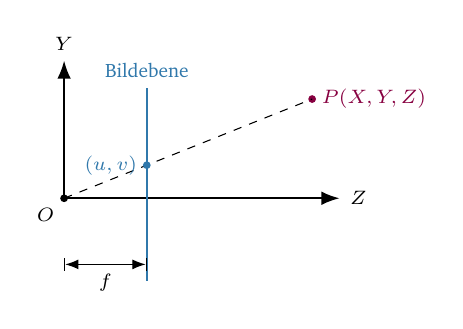
\begin{tikzpicture}[scale=0.7, >=Latex]
      % Optical axis
      \draw[->, thick] (0,0) -- (5,0) node[right]{\scriptsize $Z$};
      \draw[->, thick] (0,0) -- (0,2.5) node[above]{\scriptsize $Y$};
      % Image plane
      \draw[fbblau, thick] (1.5,-1.5) -- (1.5,2) node[above]{\scriptsize Bildebene};
      % Object point
      \fill[blackberry] (4.5,1.8) circle(2pt) node[right]{\scriptsize $P(X,Y,Z)$};
      % Projection line
      \draw[dashed] (0,0) -- (4.5,1.8);
      % Image point
      \fill[fbblau] (1.5,0.6) circle(2pt) node[left]{\scriptsize $(u,v)$};
      % Focal length
      \draw[|<->|] (0,-1.2) -- (1.5,-1.2) node[midway,below]{\scriptsize $f$};
      % Camera center
      \fill (0,0) circle(2pt) node[below left]{\scriptsize $O$};
    \end{tikzpicture}
  \end{column}
\end{columns}

\end{frame}


% -----------------------------------------------------------
\begin{frame}{Signalcharakteristika}

Kein Sensor liefert perfekte Daten. Typische Störeinflüsse:

\vspace{2mm}
\begin{columns}[T]
  \begin{column}{0.30\textwidth}
    \textbf{Rauschen}
    \begin{itemize}
      \item Gaussian Noise:
            $n \sim \mathcal{N}(0, \sigma^2)$
      \item Signal-Rausch-Verhältnis (SNR)
      \item Thermisches Rauschen,\\Quantisierungsrauschen
    \end{itemize}
  \end{column}

  \begin{column}{0.30\textwidth}
    \textbf{Bias \& Drift}
    \begin{itemize}
      \item Konstanter Offset:\\
            $\hat{x} = x + b$
      \item Drift: $b(t)$ ändert sich
            langsam über Zeit
      \item Besonders kritisch bei\\
            Gyroskopen (IMU)
    \end{itemize}
  \end{column}

  \begin{column}{0.30\textwidth}
    \textbf{Quantisierung (ADC)}
    \begin{itemize}
      \item Analog $\rightarrow$ Digital
      \item $n$ Bit $\Rightarrow$ $2^n$ Stufen
      \item Auflösung:\\
            $\Delta = \frac{V_\mathrm{ref}}{2^n}$
      \item 10-Bit ADC bei $\SI{3.3}{V}$:\\
            $\Delta \approx \SI{3.2}{mV}$
    \end{itemize}
  \end{column}
\end{columns}

\end{frame}


% -----------------------------------------------------------
\begin{frame}{Abtastung: Nyquist-Shannon-Theorem}

\begin{block}{Abtasttheorem}
  Ein Signal mit maximaler Frequenz $f_\mathrm{max}$ kann exakt
  rekonstruiert werden, wenn die Abtastrate
  $f_s > 2 \cdot f_\mathrm{max}$ beträgt.
\end{block}

\vspace{2mm}
\begin{columns}[T]
  \begin{column}{0.55\textwidth}
    \textbf{Aliasing:} Wird zu langsam abgetastet
    ($f_s \le 2 f_\mathrm{max}$), erscheinen hochfrequente
    Komponenten als niederfrequente \warn{Geistersignale}.

    \vspace{2mm}
    \textbf{Praxis:}
    \begin{itemize}
      \item IMU: typisch $\SI{100}{Hz}$ -- $\SI{1000}{Hz}$
      \item Lidar: $\SI{5}{Hz}$ -- $\SI{40}{Hz}$ (Scanrate)
      \item Kamera: $\SI{30}{Hz}$ -- $\SI{60}{Hz}$ (Framerate)
    \end{itemize}
  \end{column}
  \begin{column}{0.40\textwidth}
    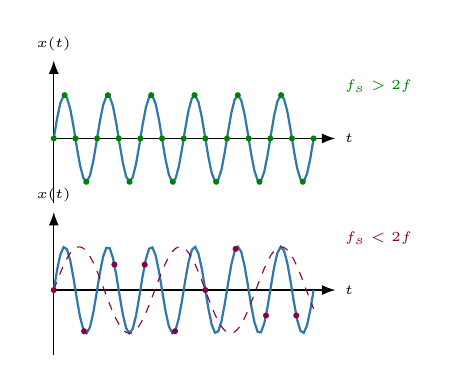
\begin{tikzpicture}[scale=0.55, >=Latex]
      % Original signal
      \draw[->] (0,0) -- (6.5,0) node[right]{\tiny $t$};
      \draw[->] (0,-1.5) -- (0,1.8) node[above]{\tiny $x(t)$};
      \draw[fbblau, thick, domain=0:6, samples=80]
        plot(\x, {sin(360*\x)});
      % Samples (good)
      \foreach \x in {0,0.25,...,6} {
        \fill[dkgreen] (\x, {sin(360*\x)}) circle(2pt);
      }
      \node[anchor=west] at (6.5,1.2) {\tiny\color{dkgreen} $f_s > 2f$};
      % Bad samples
      \begin{scope}[yshift=-3.5cm]
        \draw[->] (0,0) -- (6.5,0) node[right]{\tiny $t$};
        \draw[->] (0,-1.5) -- (0,1.8) node[above]{\tiny $x(t)$};
        \draw[fbblau, thick, domain=0:6, samples=80]
          plot(\x, {sin(360*\x)});
        \foreach \x in {0,0.7,...,6} {
          \fill[blackberry] (\x, {sin(360*\x)}) circle(2pt);
        }
        \draw[blackberry, dashed, domain=0:6, samples=80]
          plot(\x, {sin(360*0.4286*\x)});
        \node[anchor=west] at (6.5,1.2) {\tiny\color{blackberry} $f_s < 2f$};
      \end{scope}
    \end{tikzpicture}
  \end{column}
\end{columns}

\end{frame}


% -----------------------------------------------------------
\begin{frame}{Rauschen -- Warum ist es normalverteilt?}

\textbf{Zentraler Grenzwertsatz (Central Limit Theorem):}

Seien $X_1, X_2, \ldots, X_n$ unabhängige Zufallsvariablen mit
$\mathrm{E}[X_i] = \mu_i$ und $\mathrm{Var}[X_i] = \sigma_i^2$.
Dann konvergiert die Summe
\[
  S_n = \sum_{i=1}^{n} X_i
\]
für $n \to \infty$ gegen eine \hl{Normalverteilung} -- unabhängig
von der Verteilung der einzelnen $X_i$.

\vspace{2mm}
\textbf{Anwendung auf Sensoren:}
\begin{itemize}
  \item Ein Messwert wird von vielen kleinen, unabhängigen
        Störquellen beeinflusst (Temperatur, Elektronik,
        Quantisierung, Vibrationen, \ldots)
  \item Jede Störquelle $X_i$ hat eigene Verteilung
  \item Deren Summe $\Rightarrow$ Gauß-Verteilung:
        $n \sim \mathcal{N}(0, \sigma^2)$
\end{itemize}

\end{frame}


% -----------------------------------------------------------
\begin{frame}{Varianzreduktion durch Mittelung}

\textbf{Gesetz der großen Zahlen -- quantitativ:}

Seien $X_1, \ldots, X_N$ i.i.d.\ mit $\mathrm{E}[X_i] = \mu$ und
$\mathrm{Var}[X_i] = \sigma^2$. Der Mittelwert ist
\[
  \bar{X}_N = \frac{1}{N}\sum_{i=1}^{N} X_i
\]

\pause
\textbf{Erwartungswert:}
$\mathrm{E}[\bar{X}_N] = \frac{1}{N}\sum_{i=1}^N \mathrm{E}[X_i]
  = \mu$ \quad (unverzerrter Schätzer)

\pause
\textbf{Varianz:}
\[
  \mathrm{Var}[\bar{X}_N]
  = \mathrm{Var}\!\left[\frac{1}{N}\sum_{i=1}^N X_i\right]
  = \frac{1}{N^2}\sum_{i=1}^N \mathrm{Var}[X_i]
  = \frac{N\,\sigma^2}{N^2}
  = \frac{\sigma^2}{N}
\]

\pause
\begin{block}{Kernaussage}
  Mittelung über $N$ Messwerte reduziert die Varianz um den Faktor $N$.\\
  $\Rightarrow$ \textbf{Gleitender Mittelwert} = direkter Einsatz dieses Prinzips!
\end{block}

\end{frame}


% -----------------------------------------------------------
\begin{frame}{Vom Gesetz der großen Zahlen zum Moving Average}

\textbf{Moving Average als Fenster über die letzten $N$ Werte:}
\[
  y[n] = \frac{1}{N}\sum_{k=0}^{N-1} x[n-k]
\]

\vspace{1mm}
Falls $x[n] = s[n] + \epsilon[n]$ mit Signal $s$ und Rauschen
$\epsilon[n] \sim \mathcal{N}(0, \sigma^2)$:

\vspace{1mm}
\begin{columns}[T]
  \begin{column}{0.48\textwidth}
    \textbf{Signal bleibt erhalten} (falls $s$ langsam):
    \[
      \mathrm{E}[y[n]] \approx s[n]
    \]
    (Annahme: $s$ ändert sich wenig im Fenster)
  \end{column}
  \begin{column}{0.48\textwidth}
    \textbf{Rauschen wird reduziert:}
    \[
      \mathrm{Var}[y[n]] = \frac{\sigma^2}{N}
    \]
    Standardabweichung: $\sigma_y = \frac{\sigma}{\sqrt{N}}$
  \end{column}
\end{columns}

\vspace{3mm}
\begin{alertblock}{Trade-off}
  Größeres $N$ $\Rightarrow$ bessere Glättung, \textbf{aber}:
  Verzögerung $\frac{N-1}{2}$ Samples und Verlust schneller Signaländerungen.
  $\Rightarrow$ $N$ muss zum System passen!
\end{alertblock}

\end{frame}


% ============================================================
\section{Signalverarbeitung}
% ============================================================

% -----------------------------------------------------------
\begin{frame}[fragile]{Filter -- Grundlagen}

Rohe Sensordaten sind verrauscht $\Rightarrow$ \hl{Filterung} nötig.

\vspace{3mm}
\begin{columns}[T]
  \begin{column}{0.48\textwidth}
    \textbf{Moving Average (Gleitender Mittelwert):}
    \[
      y[n] = \frac{1}{N}\sum_{k=0}^{N-1} x[n-k]
    \]
    \begin{itemize}
      \item Einfach zu implementieren
      \item Glättet Rauschen
      \item Verzögerung: $\frac{N-1}{2}$ Samples
    \end{itemize}
  \end{column}
  \begin{column}{0.48\textwidth}
    \textbf{Low-Pass / High-Pass (1.\ Ordnung):}
    \[
      y[n] = \alpha \cdot x[n] + (1-\alpha) \cdot y[n-1]
    \]
    \begin{itemize}
      \item $\alpha \in (0,1]$: Glättungsfaktor
      \item $\alpha$ klein $\Rightarrow$ starke Glättung
      \item High-Pass: $y_\mathrm{HP} = x - y_\mathrm{LP}$
    \end{itemize}
  \end{column}
\end{columns}

\vspace{3mm}
\begin{exampleblock}{Implementierung (C)}
\begin{lstlisting}[language=C, numbers=none, frame=none, backgroundcolor={}]
float lp_filter(float x, float y_prev, float alpha) {
    return alpha * x + (1.0f - alpha) * y_prev;
}
\end{lstlisting}
\vspace{-2mm}
\end{exampleblock}

\end{frame}


% -----------------------------------------------------------
\begin{frame}{Low-Pass-Filter -- Herleitung aus der Physik}

\textbf{Analogie:} RC-Tiefpassfilter (Elektronik).

Die Spannung über dem Kondensator folgt der DGL:
\[
  RC \, \frac{dy}{dt} + y(t) = x(t)
\]

\textbf{Diskretisierung} (Euler-Vorwärts, Schrittweite $\Delta t$):
\[
  RC \, \frac{y[n] - y[n-1]}{\Delta t} + y[n] = x[n]
\]

\pause
Umstellen nach $y[n]$:
\[
  y[n]\left(1 + \frac{RC}{\Delta t}\right) = x[n] + \frac{RC}{\Delta t}\,y[n-1]
\]
\[
  y[n] = \underbrace{\frac{\Delta t}{RC + \Delta t}}_{\alpha}\,x[n]
       + \underbrace{\frac{RC}{RC + \Delta t}}_{1-\alpha}\,y[n-1]
\]

\pause
\begin{block}{Ergebnis: Exponential Moving Average (EMA)}
  $y[n] = \alpha \cdot x[n] + (1-\alpha) \cdot y[n-1]$
  mit $\alpha = \frac{\Delta t}{RC + \Delta t} \in (0,1)$
\end{block}

\end{frame}


% -----------------------------------------------------------
\begin{frame}{Low-Pass: Frequenzverhalten und $\alpha$}

\textbf{Zeitkonstante:} $\tau = RC$ bestimmt die Grenzfrequenz
$f_c = \frac{1}{2\pi\tau}$.

\vspace{1mm}
\begin{columns}[T]
  \begin{column}{0.48\textwidth}
    \textbf{$\alpha$ groß} (z.\,B. $0.8$):
    \begin{itemize}\setlength{\itemsep}{0pt}\setlength{\parskip}{0pt}
      \item $\tau$ klein $\Rightarrow$ $f_c$ hoch
      \item Wenig Glättung, schnelle Reaktion
      \item Mehr Rauschen durchgelassen
    \end{itemize}
  \end{column}
  \begin{column}{0.48\textwidth}
    \textbf{$\alpha$ klein} (z.\,B. $0.05$):
    \begin{itemize}\setlength{\itemsep}{0pt}\setlength{\parskip}{0pt}
      \item $\tau$ groß $\Rightarrow$ $f_c$ niedrig
      \item Starke Glättung, langsame Reaktion
      \item Rauschen stark gedämpft
    \end{itemize}
  \end{column}
\end{columns}

\vspace{1mm}
\textbf{High-Pass:}
$y_\mathrm{HP}[n] = x[n] - y_\mathrm{LP}[n]$
-- lässt schnelle Änderungen durch, blockiert Drift ($\Rightarrow$ Gyroskop!).

\vspace{1mm}
\begin{exampleblock}{Complementary Filter = LP auf Acc + HP auf Gyro}
  \vspace{-2mm}Genau das nutzt der Complementary Filter (kommt gleich).\vspace{-2mm}
\end{exampleblock}

\end{frame}


% -----------------------------------------------------------
\begin{frame}{Hidden Markov Model -- Grundstruktur}

\textbf{Idee:} Es gibt einen \hl{verborgenen Zustand} $x_k$, den wir nicht direkt
sehen -- nur über verrauschte \textbf{Beobachtungen} $z_k$.

\vspace{2mm}
\begin{center}
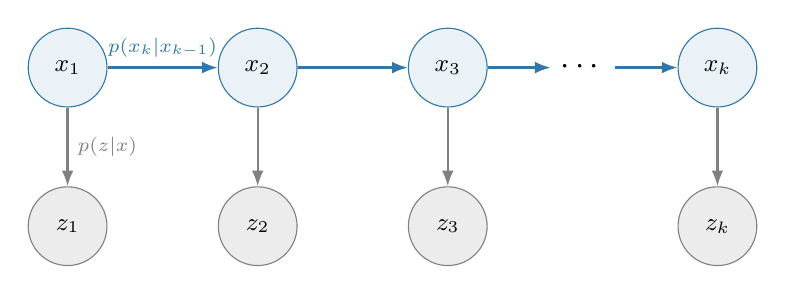
\begin{tikzpicture}[
    node distance=14mm,
    state/.style={circle, draw=fbblau, fill=fbblau!10,
                  minimum size=10mm, font=\small},
    obs/.style={circle, draw=gray, fill=gray!15,
                minimum size=10mm, font=\small},
    arr/.style={-{Latex[length=2mm]}, thick, fbblau},
    oarr/.style={-{Latex[length=2mm]}, thick, gray}
  ]
  \node[state] (x1) {$x_1$};
  \node[state, right=of x1] (x2) {$x_2$};
  \node[state, right=of x2] (x3) {$x_3$};
  \node[right=8mm of x3, font=\large] (dots) {$\cdots$};
  \node[state, right=8mm of dots] (xk) {$x_k$};

  \node[obs, below=10mm of x1] (z1) {$z_1$};
  \node[obs, below=10mm of x2] (z2) {$z_2$};
  \node[obs, below=10mm of x3] (z3) {$z_3$};
  \node[obs, below=10mm of xk] (zk) {$z_k$};

  \draw[arr] (x1) -- (x2) node[midway, above, font=\scriptsize] {$p(x_k|x_{k-1})$};
  \draw[arr] (x2) -- (x3);
  \draw[arr] (x3) -- (dots);
  \draw[arr] (dots) -- (xk);

  \draw[oarr] (x1) -- (z1) node[midway, right, font=\scriptsize] {$p(z|x)$};
  \draw[oarr] (x2) -- (z2);
  \draw[oarr] (x3) -- (z3);
  \draw[oarr] (xk) -- (zk);
\end{tikzpicture}
\end{center}

\vspace{1mm}
\textbf{Zwei Grundannahmen} (Markov-Eigenschaft):
\begin{enumerate}\setlength{\itemsep}{0pt}
  \item $x_k$ hängt \emph{nur} von $x_{k-1}$ ab: \;
        $p(x_k | x_1, \ldots, x_{k-1}) = p(x_k | x_{k-1})$
  \item $z_k$ hängt \emph{nur} von $x_k$ ab: \;
        $p(z_k | x_1, \ldots, x_k) = p(z_k | x_k)$
\end{enumerate}

\end{frame}


% -----------------------------------------------------------
\begin{frame}{Vom HMM zum Kalman-Filter}

\textbf{Ein HMM wird durch drei Größen definiert:}

\vspace{1mm}
\begin{columns}[T]
  \begin{column}{0.48\textwidth}
    \textbf{Diskretes HMM} (endliche Zustände):
    \begin{itemize}\setlength{\itemsep}{1pt}
      \item Transition: $A_{ij} = p(x_k{=}j \mid x_{k-1}{=}i)$
      \item Emission: $B_{jm} = p(z_k{=}m \mid x_k{=}j)$
      \item Inferenz: Forward-Algorithmus\\
            $\alpha_k(j) = p(z_k|x_k{=}j)\!\sum_i \alpha_{k-1}(i)\,A_{ij}$
    \end{itemize}
  \end{column}
  \begin{column}{0.48\textwidth}
    \textbf{Kontinuierliches HMM} (= Kalman!):
    \begin{itemize}\setlength{\itemsep}{1pt}
      \item Transition: $x_k = A\,x_{k-1} + w_k$\\
            {\scriptsize $\Leftrightarrow\; p(x_k|x_{k-1}) = \mathcal{N}(Ax_{k-1},\, Q)$}
      \item Emission: $z_k = H\,x_k + v_k$\\
            {\scriptsize $\Leftrightarrow\; p(z_k|x_k) = \mathcal{N}(Hx_k,\, R)$}
      \item Inferenz: \textbf{Kalman-Filter}\\
            {\scriptsize Summe $\to$ Integral, exakt lösbar!}
    \end{itemize}
  \end{column}
\end{columns}

\vspace{2mm}
\begin{block}{Der entscheidende Zusammenhang}
  \vspace{-2mm}
  \begin{center}
  \renewcommand{\arraystretch}{1.2}
  \begin{tabular}{lcc}
    & \textbf{Diskret} & \textbf{Kontinuierlich (Gauß)} \\\hline
    Zustand & endlich: $x \in \{1,\ldots,N\}$ & $x \in \R^n$ \\
    Forward-Variable & $\alpha_k(j)$ (Vektor) & $\mathcal{N}(\hat{x}_k, P_k)$ \\
    Prädiktion & Matrix-Vektor $A\,\alpha$ & $\hat{x}^- = A\hat{x},\; P^- = APA^T\!+Q$ \\
    Update & $\alpha \cdot B$ (elementweise) & Kalman-Gain $K$, Innovation
  \end{tabular}
  \end{center}
  \vspace{-2mm}
\end{block}

\end{frame}


% -----------------------------------------------------------
\begin{frame}{Bayes-Filter -- Das allgemeine Prinzip}

\textbf{Grundidee:} Zustandsschätzung als \hl{probabilistisches Schließen}.

\vspace{2mm}
Gegeben: bisherige Schätzung $p(\mathbf{x}_{k-1} | \mathbf{z}_{1:k-1})$, neue Messung $\mathbf{z}_k$.

\vspace{2mm}
\textbf{Bayes-Filter in zwei Schritten:}
\begin{enumerate}
  \item \textbf{Prädiktion} (Chapman-Kolmogorov):
        \[
          p(\mathbf{x}_k | \mathbf{z}_{1:k-1})
          = \int p(\mathbf{x}_k | \mathbf{x}_{k-1})\;
                p(\mathbf{x}_{k-1} | \mathbf{z}_{1:k-1})\;d\mathbf{x}_{k-1}
        \]
  \item \textbf{Update} (Bayes'sche Regel):
        \[
          p(\mathbf{x}_k | \mathbf{z}_{1:k})
          = \frac{p(\mathbf{z}_k | \mathbf{x}_k)\;
                  p(\mathbf{x}_k | \mathbf{z}_{1:k-1})}
                 {p(\mathbf{z}_k | \mathbf{z}_{1:k-1})}
        \]
\end{enumerate}

\pause
\vspace{1mm}
\begin{block}{Kalman-Filter = Bayes-Filter mit zwei Annahmen}
  \begin{enumerate}
    \item \textbf{Lineares} Systemmodell: $\mathbf{x}_k = A\mathbf{x}_{k-1} + B\mathbf{u}_k + \mathbf{w}_k$
    \item \textbf{Gauß'sches} Rauschen: $\mathbf{w}_k \sim \mathcal{N}(\mathbf{0},Q)$, \;
          $\mathbf{v}_k \sim \mathcal{N}(\mathbf{0},R)$
  \end{enumerate}
  Unter diesen Annahmen bleibt die Verteilung \emph{immer} Gauß'sch --
  die Integrale lassen sich \emph{analytisch} lösen!
\end{block}

\end{frame}


% -----------------------------------------------------------
\begin{frame}{Kalman-Filter -- Das Systemmodell}

\textbf{Ausgangspunkt:} Lineares zeitdiskretes System mit Rauschen.

\vspace{2mm}
\begin{block}{Zustandsgleichung (Prozessmodell)}
  $\mathbf{x}_k = A\,\mathbf{x}_{k-1} + B\,\mathbf{u}_k + \mathbf{w}_k$
  \quad mit $\mathbf{w}_k \sim \mathcal{N}(\mathbf{0}, Q)$
\end{block}
\begin{block}{Messgleichung (Beobachtungsmodell)}
  $\mathbf{z}_k = H\,\mathbf{x}_k + \mathbf{v}_k$
  \quad mit $\mathbf{v}_k \sim \mathcal{N}(\mathbf{0}, R)$
\end{block}

\vspace{2mm}
\textbf{Die Matrizen im Detail:}
\begin{tabular}{lll}
  $\mathbf{x}_k \in \R^n$ & Zustandsvektor & (was wir schätzen wollen) \\
  $\mathbf{u}_k \in \R^m$ & Steuervektor & (bekannte Eingabe) \\
  $\mathbf{z}_k \in \R^p$ & Messvektor & (was der Sensor liefert) \\
  $A \in \R^{n \times n}$  & Systemmatrix & (wie sich der Zustand entwickelt) \\
  $B \in \R^{n \times m}$  & Steuermatrix & (Einfluss der Steuerung) \\
  $H \in \R^{p \times n}$  & Messmatrix & (Zusammenhang Zustand $\leftrightarrow$ Messung)
\end{tabular}

\end{frame}


% -----------------------------------------------------------
\begin{frame}{Kalman-Filter -- Kovarianzmatrizen}

\textbf{Was ist eine Kovarianzmatrix?}

Für einen Zufallsvektor $\mathbf{x} = (x_1, \ldots, x_n)^T$:
\[
  P = \mathrm{Cov}[\mathbf{x}] = \mathrm{E}[(\mathbf{x} - \bm{\mu})(\mathbf{x} - \bm{\mu})^T]
  = \begin{bmatrix}
    \sigma_{x_1}^2 & \mathrm{cov}(x_1,x_2) & \cdots \\
    \mathrm{cov}(x_2,x_1) & \sigma_{x_2}^2 & \cdots \\
    \vdots & \vdots & \ddots
  \end{bmatrix}
\]

\vspace{1mm}
\textbf{Drei Kovarianzmatrizen im Kalman-Filter:}

\begin{itemize}
  \item $P_k \in \R^{n\times n}$: \hl{Schätzunsicherheit} --
        wie unsicher ist unser aktueller Zustandsschätzer?
        Diagonale = Varianz jeder Zustandsgröße.
  \item $Q \in \R^{n\times n}$: \hl{Prozessrauschen} --
        wie ungenau ist unser Modell?
        Größeres $Q$ $\Rightarrow$ Filter vertraut dem Modell weniger.
  \item $R \in \R^{p\times p}$: \hl{Messrauschen} --
        wie ungenau ist der Sensor?
        Größeres $R$ $\Rightarrow$ Filter vertraut der Messung weniger.
\end{itemize}

\end{frame}


% -----------------------------------------------------------
\begin{frame}{Kalman-Filter -- Herleitung der Prädiktion}

\textbf{Schritt 1: Vorhersage des Zustands.}

Wenn wir das Systemmodell kennen, können wir vorhersagen:
\[
  \hat{\mathbf{x}}_{k|k-1} = A\,\hat{\mathbf{x}}_{k-1} + B\,\mathbf{u}_k
\]

\textbf{Wie entwickelt sich die Unsicherheit?}

\pause
Die Kovarianz transformiert sich durch lineare Abbildung $A$ als:
\[
  \mathrm{Cov}[A\mathbf{x}] = A\,\mathrm{Cov}[\mathbf{x}]\,A^T
\]
(Dies folgt direkt aus $\mathrm{E}[(A\mathbf{x})(A\mathbf{x})^T] = A\,\mathrm{E}[\mathbf{x}\mathbf{x}^T]\,A^T$.)

\pause
Dazu kommt das Prozessrauschen $Q$:
\[
  \boxed{P_{k|k-1} = A\,P_{k-1}\,A^T + Q}
\]

\begin{alertblock}{Intuition}
  Die Unsicherheit \emph{wächst} bei jeder Prädiktion -- wir verlieren
  Information, weil das Modell nicht perfekt ist.
\end{alertblock}

\end{frame}


% -----------------------------------------------------------
\begin{frame}{Kalman-Filter -- Herleitung des Updates}

\textbf{Schritt 2: Korrektur mit der Messung.}

Die \hl{Innovation} (Überraschung der Messung):
\[
  \tilde{\mathbf{y}}_k = \mathbf{z}_k - H\,\hat{\mathbf{x}}_{k|k-1}
\]

\pause
\textbf{Innovationskovarianz} (wie unsicher ist die Überraschung?):
\[
  S_k = H\,P_{k|k-1}\,H^T + R
\]

\pause
\textbf{Kalman-Gain} (optimale Gewichtung):
\[
  \boxed{K_k = P_{k|k-1}\,H^T\,S_k^{-1}}
\]

\pause
\textbf{Update-Gleichungen:}
\[
  \boxed{\hat{\mathbf{x}}_k = \hat{\mathbf{x}}_{k|k-1} + K_k\,\tilde{\mathbf{y}}_k}
  \qquad
  \boxed{P_k = (I - K_k\,H)\,P_{k|k-1}}
\]

\vspace{1mm}
Der Kalman-Gain minimiert den mittleren quadratischen Fehler
$\mathrm{E}[\|\mathbf{x}_k - \hat{\mathbf{x}}_k\|^2]$ -- er ist
\hl{optimal} für lineare Systeme mit Gauß'schem Rauschen.

\end{frame}


% -----------------------------------------------------------
\begin{frame}{Kalman-Filter -- Intuition des Kalman-Gain}

\textbf{Was macht $K_k = P_{k|k-1}\,H^T\,(H\,P_{k|k-1}\,H^T + R)^{-1}$?}

\vspace{3mm}
\begin{columns}[T]
  \begin{column}{0.48\textwidth}
    \textbf{Fall 1: $R$ klein} (Sensor genau)
    \begin{itemize}
      \item $S_k \approx H P_{k|k-1} H^T$
      \item $K_k$ wird groß
      \item $\hat{x}_k \approx$ Messung
    \end{itemize}
    $\Rightarrow$ Filter vertraut dem Sensor.
  \end{column}
  \begin{column}{0.48\textwidth}
    \textbf{Fall 2: $P_{k|k-1}$ klein} (Modell sicher)
    \begin{itemize}
      \item Zähler $P_{k|k-1} H^T$ wird klein
      \item $K_k \rightarrow 0$
      \item $\hat{x}_k \approx$ Prädiktion
    \end{itemize}
    $\Rightarrow$ Filter vertraut dem Modell.
  \end{column}
\end{columns}

\vspace{4mm}
\begin{center}
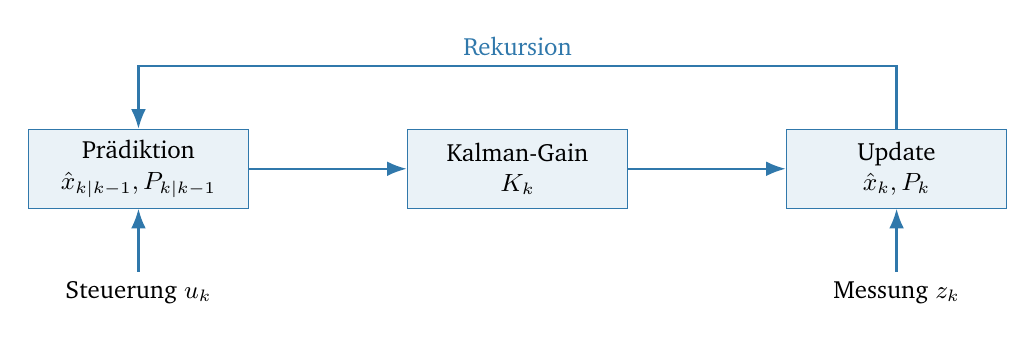
\begin{tikzpicture}[
    node distance=12mm and 20mm,
    box/.style={rectangle, draw=fbblau, fill=fbblau!10,
                minimum width=28mm, minimum height=10mm,
                text centered, font=\small, align=center},
    arr/.style={-{Latex[length=2.5mm]}, thick, fbblau}
  ]
  \node[box] (pred) {Pr\"adiktion\\ $\hat{x}_{k|k-1}, P_{k|k-1}$};
  \node[box, right=of pred] (gain) {Kalman-Gain\\ $K_k$};
  \node[box, right=of gain] (upd) {Update\\ $\hat{x}_k, P_k$};
  \node[below=8mm of pred, font=\small] (u) {Steuerung $u_k$};
  \node[below=8mm of upd, font=\small]  (z) {Messung $z_k$};
  \draw[arr] (pred) -- (gain);
  \draw[arr] (gain) -- (upd);
  \draw[arr] (u) -- (pred);
  \draw[arr] (z) -- (upd);
  \draw[arr] (upd.north) -- ++(0,8mm) -| (pred.north)
    node[pos=0.25, above, font=\small]{Rekursion};
\end{tikzpicture}
\end{center}

\end{frame}


% -----------------------------------------------------------
\begin{frame}{Kalman-Filter -- Turtlebot Systemmodell}

\textbf{Zustand:} $\mathbf{x} = (x, y, \theta, v, \omega)^T$
\quad (Position, Orientierung, Geschwindigkeiten)

\vspace{2mm}
\textbf{Prozessmodell} (Differential Drive, $\Delta t$ klein):
\[
  \mathbf{x}_{k+1} = \underbrace{
    \begin{bmatrix}
      1 & 0 & 0 & \cos\theta_k\,\Delta t & 0 \\
      0 & 1 & 0 & \sin\theta_k\,\Delta t & 0 \\
      0 & 0 & 1 & 0 & \Delta t \\
      0 & 0 & 0 & 1 & 0 \\
      0 & 0 & 0 & 0 & 1
    \end{bmatrix}
  }_{f(\mathbf{x}_k)} \mathbf{x}_k + \mathbf{w}_k
\]

\pause
\begin{alertblock}{Nichtlinearität!}
  \vspace{-2mm}Matrix hängt von $\theta_k$ ab $\Rightarrow$ \warn{nichtlinear} -- Standard-Kalman nicht direkt anwendbar!\vspace{-2mm}
\end{alertblock}

\vspace{0.5mm}
\textbf{Messmodell} (Encoder: $v, \omega$; Lidar: $x,y$):\;
$\mathbf{z}_k = H\,\mathbf{x}_k + \mathbf{v}_k$\; mit\;
$H = \begin{bsmallmatrix} 1&0&0&0&0 \\ 0&1&0&0&0 \\ 0&0&0&1&0 \\ 0&0&0&0&1 \end{bsmallmatrix}$

\end{frame}


% -----------------------------------------------------------
\begin{frame}{Turtlebot -- Kovarianzmatrizen konkret}

\textbf{Prozessrauschen $Q$} -- Unsicherheit des Bewegungsmodells:
\[
  Q = \mathrm{diag}\!\left(\sigma_x^2,\; \sigma_y^2,\; \sigma_\theta^2,\;
      \sigma_v^2,\; \sigma_\omega^2\right)
\]
Typisch: $\sigma_x = \sigma_y \approx \SI{0.01}{m}$, \;
$\sigma_\theta \approx \SI{0.01}{rad}$, \;
$\sigma_v \approx \SI{0.05}{m/s}$

\vspace{3mm}
\textbf{Messrauschen $R$} -- Unsicherheit der Sensoren:
\[
  R = \mathrm{diag}\!\left(\sigma_{x,\mathrm{lidar}}^2,\; \sigma_{y,\mathrm{lidar}}^2,\;
      \sigma_{v,\mathrm{enc}}^2,\; \sigma_{\omega,\mathrm{enc}}^2\right)
\]
Typisch: $\sigma_\mathrm{lidar} \approx \SI{0.05}{m}$, \;
$\sigma_\mathrm{enc} \approx \SI{0.02}{m/s}$

\vspace{3mm}
\begin{exampleblock}{Tuning-Faustregel}
  $Q$ und $R$ werden aus \textbf{Sensor-Datenblättern} und
  \textbf{experimentellen Messungen} bestimmt. Das Verhältnis $Q/R$ bestimmt,
  ob der Filter eher dem Modell oder den Sensoren vertraut.
\end{exampleblock}

\end{frame}


% -----------------------------------------------------------
\begin{frame}{Extended Kalman Filter (EKF)}

\textbf{Problem:} Turtlebot-Modell ist nichtlinear:
$\mathbf{x}_{k+1} = f(\mathbf{x}_k, \mathbf{u}_k) + \mathbf{w}_k$

\vspace{2mm}
\textbf{Idee:} Linearisiere $f$ in jedem Zeitschritt um den aktuellen
Schätzwert $\hat{\mathbf{x}}_k$ mittels \hl{Jacobi-Matrix}:
\[
  F_k = \frac{\partial f}{\partial \mathbf{x}}\bigg|_{\hat{\mathbf{x}}_k}
  =
  \begin{bmatrix}
    1 & 0 & -v_k\sin\theta_k\,\Delta t & \cos\theta_k\,\Delta t & 0 \\
    0 & 1 & \phantom{-}v_k\cos\theta_k\,\Delta t & \sin\theta_k\,\Delta t & 0 \\
    0 & 0 & 1 & 0 & \Delta t \\
    0 & 0 & 0 & 1 & 0 \\
    0 & 0 & 0 & 0 & 1
  \end{bmatrix}
\]

\pause
\textbf{EKF-Gleichungen} (wie Kalman, aber $A \to F_k$):
\begin{align*}
  \text{Prädiktion:}\quad
    & \hat{\mathbf{x}}_{k|k-1} = f(\hat{\mathbf{x}}_{k-1}, \mathbf{u}_k),
    \quad P_{k|k-1} = F_k\,P_{k-1}\,F_k^T + Q \\
  \text{Update:}\quad
    & K_k = P_{k|k-1}\,H^T\,(H\,P_{k|k-1}\,H^T + R)^{-1} \\
    & \hat{\mathbf{x}}_k = \hat{\mathbf{x}}_{k|k-1} + K_k\,(z_k - H\,\hat{\mathbf{x}}_{k|k-1})
\end{align*}

\end{frame}


% -----------------------------------------------------------
\begin{frame}{EKF -- Zusammenfassung und Grenzen}

\begin{columns}[T]
  \begin{column}{0.48\textwidth}
    \textbf{Vorteile des EKF:}
    \begin{itemize}\setlength{\itemsep}{0pt}\setlength{\parskip}{0pt}
      \item Funktioniert für nichtlineare Systeme
      \item Standardverfahren in der Robotik
      \item Effizient (nur Matrixoperationen)
      \item Gut verstanden, viele Bibliotheken
    \end{itemize}
  \end{column}
  \begin{column}{0.48\textwidth}
    \textbf{Grenzen des EKF:}
    \begin{itemize}\setlength{\itemsep}{0pt}\setlength{\parskip}{0pt}
      \item Linearisierung nur lokal gültig
      \item Kann bei starker Nichtlinearität divergieren
      \item Gauß-Annahme kann verletzt sein
      \item Jacobi-Matrizen analytisch nötig
    \end{itemize}
  \end{column}
\end{columns}

\vspace{1mm}
\begin{block}{Alternativen bei starker Nichtlinearität}
  \vspace{-2mm}
  \begin{itemize}\setlength{\itemsep}{0pt}
    \item \textbf{UKF:} Sigma-Punkte statt Linearisierung
    \item \textbf{Partikelfilter:} Monte-Carlo-Sampling, keine Gauß-Annahme nötig
  \end{itemize}
  \vspace{-2mm}
\end{block}

\end{frame}


% -----------------------------------------------------------
\begin{frame}{Complementary Filter (IMU)}

\textbf{Problem:} Gyroskop liefert gute \emph{kurzfristige} Orientierung
(aber driftet), Beschleunigungssensor liefert stabile \emph{langfristige}
Neigung (aber verrauscht).

\vspace{3mm}
\begin{block}{Complementary Filter}
  \[
    \theta_k = \alpha \cdot (\theta_{k-1} + \omega_k \cdot \Delta t)
             + (1-\alpha) \cdot \theta_\mathrm{acc,k}
  \]
  mit $\alpha \approx 0.98$ (High-Pass auf Gyro, Low-Pass auf Beschleunigung).
\end{block}

\vspace{3mm}
\begin{itemize}
  \item \textbf{Vorteil:} Extrem einfach, kaum Rechenaufwand
  \item \textbf{Nachteil:} Nicht optimal, kein Modell der Unsicherheit
  \item \textbf{Einsatz:} Drohnen, Turtlebot, schnelle Prototypen
\end{itemize}

\end{frame}


% ============================================================
\section{Zustandsschätzung}
% ============================================================

% -----------------------------------------------------------
\begin{frame}{Pose eines Roboters}

Die \hl{Pose} beschreibt Position und Orientierung in der Ebene:
\[
  \mathbf{q} = \begin{bmatrix} x \\ y \\ \theta \end{bmatrix}
  \in \R^2 \times (-\pi, \pi]
\]

\begin{columns}[T]
  \begin{column}{0.50\textwidth}
    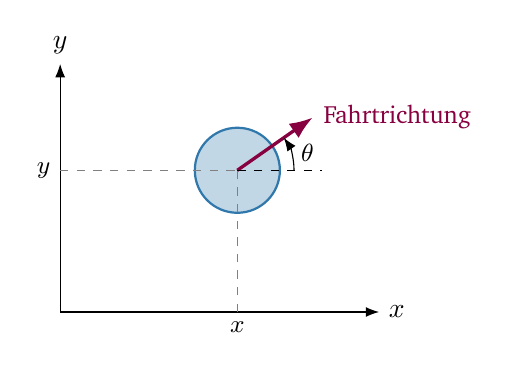
\begin{tikzpicture}[scale=0.9, >=Latex]
      \draw[->] (0,0) -- (4.5,0) node[right]{$x$};
      \draw[->] (0,0) -- (0,3.5) node[above]{$y$};
      % Robot
      \fill[fbblau!30] (2.5,2) circle(6mm);
      \draw[fbblau, thick] (2.5,2) circle(6mm);
      \draw[->, very thick, blackberry] (2.5,2) -- ++(35:1.3)
        node[right]{\small Fahrtrichtung};
      % Angle
      \draw[dashed] (2.5,2) -- ++(1.2,0);
      \draw[->] (3.3,2) arc(0:35:0.8) node[midway, right]{\small $\theta$};
      % Coordinates
      \draw[dashed, gray] (2.5,0) -- (2.5,2);
      \draw[dashed, gray] (0,2) -- (2.5,2);
      \node[below] at (2.5,0) {\small $x$};
      \node[left] at (0,2) {\small $y$};
    \end{tikzpicture}
  \end{column}
  \begin{column}{0.45\textwidth}
    \textbf{Warum reicht $(x,y)$ nicht?}
    \begin{itemize}
      \item Roboter muss wissen, \emph{wohin} er schaut
      \item Steuerung hängt von $\theta$ ab
      \item Sensoren sind richtungsabhängig
            (Kamera, Lidar)
    \end{itemize}
  \end{column}
\end{columns}

\end{frame}


% -----------------------------------------------------------
\begin{frame}{Odometrie -- Wheel Encoder}

\textbf{Idee:} Aus der Raddrehung auf die zurückgelegte Strecke schließen.

\vspace{2mm}
\begin{columns}[T]
  \begin{column}{0.50\textwidth}
    \textbf{Encoder-Modell:}
    \begin{itemize}
      \item Ticks pro Umdrehung: $N_\mathrm{ticks}$
      \item Radradius: $r$
      \item Strecke pro Tick: $\Delta s = \frac{2\pi r}{N_\mathrm{ticks}}$
    \end{itemize}

    \vspace{2mm}
    \textbf{Differentielle Odometrie:}
    \begin{align*}
      \Delta s &= \frac{\Delta s_L + \Delta s_R}{2} \\
      \Delta \theta &= \frac{\Delta s_R - \Delta s_L}{L}
    \end{align*}
    ($L$ = Achsabstand)
  \end{column}
  \begin{column}{0.45\textwidth}
    \begin{alertblock}{Problem: Drift!}
      Odometrie akkumuliert Fehler über die Zeit:
      \begin{itemize}
        \item Radschlupf
        \item Ungleiche Raddurchmesser
        \item Bodenunebenheiten
      \end{itemize}
      $\Rightarrow$ \textbf{Sensorfusion} nötig!
    \end{alertblock}
  \end{column}
\end{columns}

\end{frame}


% -----------------------------------------------------------
\begin{frame}{Sensorfusion}

\textbf{Ziel:} Mehrere Sensoren kombinieren, um die Schwächen
einzelner Sensoren auszugleichen.

\vspace{3mm}
\begin{center}
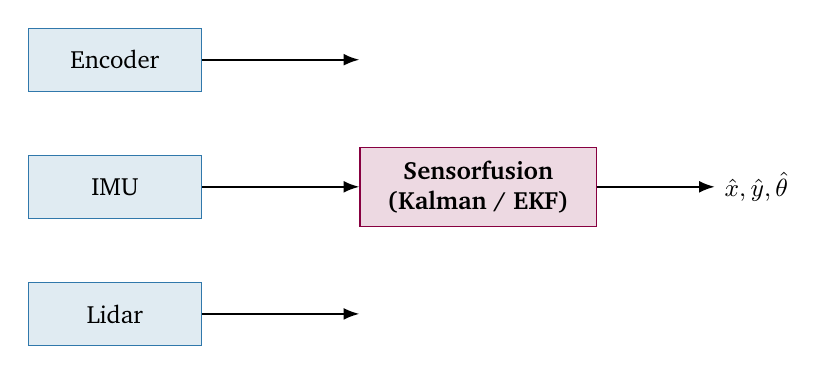
\begin{tikzpicture}[
    node distance=8mm and 14mm,
    sensor/.style={rectangle, draw=fbblau, fill=fbblau!15,
                   minimum width=22mm, minimum height=8mm,
                   font=\small},
    fuse/.style={rectangle, draw=blackberry, fill=blackberry!15,
                 minimum width=30mm, minimum height=10mm,
                 font=\small\bfseries, align=center},
    arr/.style={-{Latex[length=2mm]}, thick}
  ]
  \node[sensor] (enc)  {Encoder};
  \node[sensor, below=of enc]  (imu)  {IMU};
  \node[sensor, below=of imu]  (lid)  {Lidar};
  \node[fuse, right=20mm of imu] (fus) {Sensorfusion\\ (Kalman / EKF)};
  \node[right=15mm of fus, font=\small] (out)
    {$\hat{x}, \hat{y}, \hat{\theta}$};

  \draw[arr] (enc.east) -- (fus.west |- enc);
  \draw[arr] (imu.east) -- (fus.west);
  \draw[arr] (lid.east) -- (fus.west |- lid);
  \draw[arr] (fus) -- (out);
\end{tikzpicture}
\end{center}

\vspace{2mm}
\begin{itemize}
  \item \textbf{Encoder:} hochfrequent, aber driftet
  \item \textbf{IMU:} schnelle Dynamik, aber Gyro-Drift
  \item \textbf{Lidar:} absolut genau, aber niedrige Rate
\end{itemize}
$\Rightarrow$ Kalman-Filter gewichtet je nach Unsicherheit.

\end{frame}


% ============================================================
\section{Kinematik \& Bewegungsmodelle}
% ============================================================

% -----------------------------------------------------------
\begin{frame}{Differential Drive (Turtlebot)}

\begin{columns}[T]
  \begin{column}{0.50\textwidth}
    \textbf{Aufbau:}
    \begin{itemize}
      \item Zwei unabhängig angetriebene Räder
      \item Stützrad (passiv)
      \item Parameter: Radradius $r$, Achsabstand $L$
    \end{itemize}

    \vspace{2mm}
    \textbf{Geschwindigkeiten:}
    \begin{align*}
      v   &= \frac{r}{2}(\omega_R + \omega_L) \\
      \omega &= \frac{r}{L}(\omega_R - \omega_L)
    \end{align*}
    $\omega_R, \omega_L$: Winkelgeschwindigkeiten der Räder
  \end{column}
  \begin{column}{0.45\textwidth}
    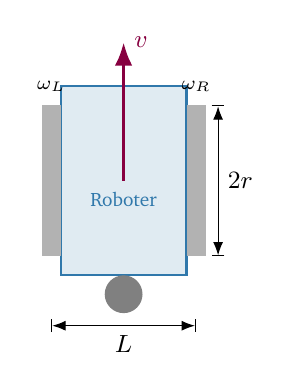
\begin{tikzpicture}[scale=0.8, >=Latex]
      % Body
      \fill[fbblau!15] (-1,-1.5) rectangle (1,1.5);
      \draw[fbblau, thick] (-1,-1.5) rectangle (1,1.5);
      % Wheels
      \fill[gray!60] (-1.3,-1.2) rectangle (-1,1.2);
      \fill[gray!60] (1,-1.2) rectangle (1.3,1.2);
      \node[font=\scriptsize] at (-1.15,1.5) {$\omega_L$};
      \node[font=\scriptsize] at (1.15,1.5) {$\omega_R$};
      % Caster
      \fill[gray] (0,-1.8) circle(3mm);
      % Direction
      \draw[->, very thick, blackberry] (0,0) -- (0,2.2)
        node[right]{\small $v$};
      % L
      \draw[|<->|] (-1.15,-2.3) -- (1.15,-2.3)
        node[midway, below]{\small $L$};
      % r
      \draw[|<->|] (1.5,-1.2) -- (1.5,1.2)
        node[midway, right]{\small $2r$};
      % Label
      \node[font=\scriptsize, fbblau] at (0,-0.3) {Roboter};
    \end{tikzpicture}
  \end{column}
\end{columns}

\end{frame}


% -----------------------------------------------------------
\begin{frame}{Forward \& Inverse Kinematics}

\begin{columns}[T]
  \begin{column}{0.48\textwidth}
    \textbf{Forward Kinematics:}\\
    $v, \omega \;\rightarrow\; x, y, \theta$

    \vspace{2mm}
    Diskretisiert ($\Delta t$ klein):
    \begin{align*}
      x_{k+1}      &= x_k + v_k \cos(\theta_k)\,\Delta t \\
      y_{k+1}      &= y_k + v_k \sin(\theta_k)\,\Delta t \\
      \theta_{k+1}  &= \theta_k + \omega_k\,\Delta t
    \end{align*}

    \emph{Gegeben:} Rad-Geschwindigkeiten\\
    \emph{Gesucht:} resultierende Pose
  \end{column}
  \begin{column}{0.48\textwidth}
    \textbf{Inverse Kinematics:}\\
    Gewünschte Bewegung $\rightarrow$ Radgeschwindigkeiten

    \vspace{2mm}
    \begin{align*}
      \omega_R &= \frac{v + \frac{L}{2}\,\omega}{r} \\[2mm]
      \omega_L &= \frac{v - \frac{L}{2}\,\omega}{r}
    \end{align*}

    \emph{Gegeben:} gewünschtes $(v, \omega)$\\
    \emph{Gesucht:} Motoransteuerung $(\omega_L, \omega_R)$
  \end{column}
\end{columns}

\end{frame}


% ============================================================
\section{Regelung (Control)}
% ============================================================

% -----------------------------------------------------------
\begin{frame}{Ohne Zustandsschätzung kein stabiler Regler}

\textbf{Warum hängen Estimation und Control zusammen?}

\vspace{2mm}
Der PID-Regler braucht den \hl{aktuellen Zustand} als Eingabe:
\[
  e(t) = x_\mathrm{soll} - \underbrace{x_\mathrm{ist}}_{\text{woher?}}
\]

Aber $x_\mathrm{ist}$ ist \emph{nie} direkt messbar -- nur über verrauschte Sensoren!

\pause
\vspace{2mm}
\begin{columns}[T]
  \begin{column}{0.48\textwidth}
    \textbf{Ohne Filter (rohe Sensordaten):}
    \begin{itemize}
      \item Rauschen geht direkt in $e(t)$
      \item $K_d \cdot \frac{de}{dt}$ verstärkt Rauschen!
      \item Regler \warn{oszilliert} oder wird instabil
    \end{itemize}
  \end{column}
  \begin{column}{0.48\textwidth}
    \textbf{Mit Kalman-Filter:}
    \begin{itemize}
      \item Geglättete, optimale Schätzung $\hat{x}$
      \item Auch Geschwindigkeit $\hat{v}$ geschätzt (nicht numerisch differenziert)
      \item Regler bekommt \hl{saubere} Eingabe
    \end{itemize}
  \end{column}
\end{columns}

\vspace{3mm}
\begin{block}{Separation Principle (LQG)}
  Für lineare Systeme mit Gauß'schem Rauschen kann man
  Zustandsschätzung (Kalman) und Regelung (LQR/PID)
  \textbf{getrennt} entwerfen -- das Gesamtsystem bleibt optimal.
\end{block}

\end{frame}


% -----------------------------------------------------------
\begin{frame}{Feedback Control -- PID-Regler}

\begin{block}{PID-Regelgesetz}
  \[
    u(t) = K_p \, e(t) + K_i \int_0^t e(\tau)\,d\tau
         + K_d \, \frac{de(t)}{dt}
  \]
  mit Regelabweichung $e(t) = x_\mathrm{soll}(t) - x_\mathrm{ist}(t)$
\end{block}

\vspace{2mm}
\begin{columns}[T]
  \begin{column}{0.55\textwidth}
    \begin{center}
    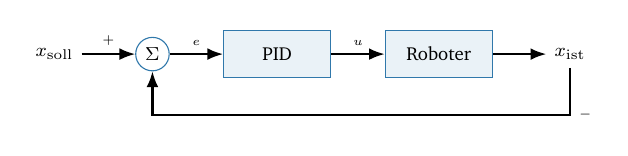
\begin{tikzpicture}[scale=0.85, every node/.style={transform shape},
        node distance=5mm and 8mm,
        box/.style={rectangle, draw=fbblau, fill=fbblau!10,
                    minimum width=16mm, minimum height=7mm,
                    text centered, font=\footnotesize},
        sum/.style={circle, draw=fbblau, inner sep=1pt,
                    minimum size=5mm, font=\footnotesize},
        arr/.style={-{Latex[length=2mm]}, thick}
      ]
      \node[font=\footnotesize] (ref) {$x_\mathrm{soll}$};
      \node[sum, right=of ref] (s) {$\Sigma$};
      \node[box, right=of s]   (pid) {PID};
      \node[box, right=of pid] (sys) {Roboter};
      \node[right=8mm of sys, font=\footnotesize] (out) {$x_\mathrm{ist}$};

      \draw[arr] (ref) -- (s) node[midway, above]{\tiny $+$};
      \draw[arr] (s)   -- (pid) node[midway, above]{\tiny $e$};
      \draw[arr] (pid) -- (sys) node[midway, above]{\tiny $u$};
      \draw[arr] (sys) -- (out);
      \draw[arr] (out.south) -- ++(0,-7mm) -| (s.south)
        node[pos=0, right]{\tiny $-$};
    \end{tikzpicture}
    \end{center}
  \end{column}
  \begin{column}{0.40\textwidth}
    \begin{itemize}
      \item $K_p$: Proportional -- reagiert auf aktuellen Fehler
      \item $K_i$: Integral -- beseitigt stationären Fehler
      \item $K_d$: Differential -- dämpft Überschwinger
    \end{itemize}
  \end{column}
\end{columns}

\end{frame}


% -----------------------------------------------------------
\begin{frame}{Trajektorienverfolgung}

\textbf{Aufgabe:} Roboter soll einem Pfad folgen
oder einen Zielpunkt $(x_g, y_g)$ erreichen.

\vspace{3mm}
\textbf{Einfache Strategie (``go-to-goal''):}
\begin{enumerate}
  \item Berechne Richtung zum Ziel:
        $\alpha = \mathrm{atan2}(y_g - y, \; x_g - x)$
  \item Regelfehler Orientierung:
        $e_\theta = \alpha - \theta$
  \item PID auf $e_\theta$ liefert $\omega$
  \item $v$ konstant oder abhängig von Distanz
\end{enumerate}

\vspace{3mm}
\begin{alertblock}{Stabilität}
  \begin{itemize}
    \item \textbf{Overshoot:} Roboter schießt über Ziel hinaus
          ($K_p$ zu groß)
    \item \textbf{Oszillation:} Pendeln um Zielpunkt ($K_d$ zu klein)
    \item \textbf{Stationärer Fehler:} Ziel wird nie ganz erreicht
          ($K_i = 0$)
  \end{itemize}
\end{alertblock}

\end{frame}


% ============================================================
\section{Lokalisierung \& Mapping (SLAM)}
% ============================================================

% -----------------------------------------------------------
\begin{frame}{Das Lokalisierungsproblem}

\begin{columns}[T]
  \begin{column}{0.55\textwidth}
    \textbf{Zwei fundamentale Fragen:}
    \begin{enumerate}
      \item \hl{Wo bin ich?} (Lokalisierung)
      \item \hl{Wie sieht die Welt aus?} (Mapping)
    \end{enumerate}

    \vspace{3mm}
    \textbf{Henne-Ei-Problem:}
    \begin{itemize}
      \item Lokalisierung braucht Karte
      \item Kartenbau braucht Position
      \item $\Rightarrow$ beides gleichzeitig: \textbf{SLAM}
    \end{itemize}
  \end{column}
  \begin{column}{0.40\textwidth}
    \textbf{Landmarken:}
    \begin{itemize}
      \item Markante Punkte in der Umgebung
      \item Wiedererkennbar (Ecken, Kanten, Objekte)
      \item Distanz + Winkel $\Rightarrow$ Triangulation
    \end{itemize}
    \vspace{2mm}
    \textbf{Occupancy Grid Map:}
    \begin{itemize}
      \item Raster: jede Zelle frei / belegt / unbekannt
      \item Aufgebaut aus Lidar-Scans
      \item Grundlage für Pfadplanung
    \end{itemize}
  \end{column}
\end{columns}

\end{frame}


% -----------------------------------------------------------
\begin{frame}{SLAM -- Simultaneous Localization and Mapping}

\begin{center}
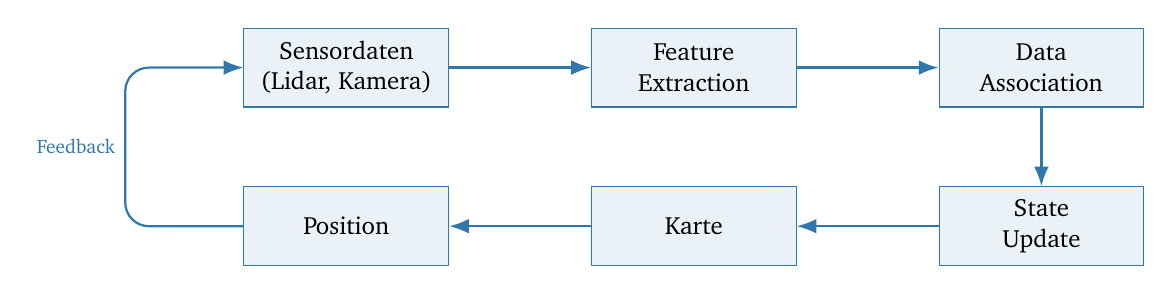
\begin{tikzpicture}[
    node distance=10mm and 18mm,
    box/.style={rectangle, draw=fbblau, fill=fbblau!10,
                minimum width=26mm, minimum height=10mm,
                text centered, font=\small, align=center},
    arr/.style={-{Latex[length=2.5mm]}, thick, fbblau}
  ]
  \node[box] (sens)  {Sensordaten\\ (Lidar, Kamera)};
  \node[box, right=of sens] (fe) {Feature\\ Extraction};
  \node[box, right=of fe]   (da) {Data\\ Association};
  \node[box, below=10mm of da]  (upd) {State\\ Update};
  \node[box, left=of upd]  (map) {Karte};
  \node[box, left=of map]  (pos) {Position};

  \draw[arr] (sens) -- (fe);
  \draw[arr] (fe)   -- (da);
  \draw[arr] (da)   -- (upd);
  \draw[arr] (upd)  -- (map);
  \draw[arr] (map)  -- (pos);
  % Feedback: route left around the outside of the diagram
  \draw[arr, rounded corners=3mm]
    (pos.west) -- ++(-15mm,0) |- (sens.west)
    node[pos=0.25, left, font=\scriptsize]{Feedback};
\end{tikzpicture}
\end{center}

\vspace{2mm}
\begin{itemize}
  \item \textbf{Feature Extraction:} Landmarken aus Sensordaten extrahieren
  \item \textbf{Data Association:} Welche beobachtete Landmarke
        entspricht welcher bekannten?
  \item \textbf{State Update:} Karte und Position gemeinsam korrigieren
        (EKF-SLAM, Partikelfilter, Graph-SLAM)
\end{itemize}

\end{frame}


% -----------------------------------------------------------
\begin{frame}{Vom EKF zu SLAM -- der wachsende Zustandsvektor}

\textbf{EKF-Lokalisierung} (bekannte Karte):
$\mathbf{x} = (x, y, \theta)^T \in \R^3$
\quad -- feste Dimension.

\pause
\vspace{2mm}
\textbf{EKF-SLAM} (unbekannte Karte): Landmarken werden Teil des Zustands!
\[
  \mathbf{x}_\mathrm{SLAM} =
  \begin{bmatrix}
    x_R \\ y_R \\ \theta_R \\
    \hline
    x_{L_1} \\ y_{L_1} \\
    \hline
    x_{L_2} \\ y_{L_2} \\
    \hline
    \vdots \\
    x_{L_M} \\ y_{L_M}
  \end{bmatrix}
  \in \R^{3 + 2M}
\]

Jede neue Landmarke erweitert den Vektor um 2 Einträge!

\pause
\vspace{1mm}
\begin{alertblock}{Skalierungsproblem}
  \vspace{-2mm}
  $P \in \R^{(3+2M) \times (3+2M)}$ wächst \warn{quadratisch}!
  Bei $M{=}1000$: ${>}\,4$ Mio.\ Einträge
  $\Rightarrow$ EKF-SLAM für große Umgebungen zu langsam.
  Alternativen: \textbf{Partikelfilter-SLAM}, \textbf{Graph-SLAM}.\vspace{-2mm}
\end{alertblock}

\end{frame}


% -----------------------------------------------------------
\begin{frame}{SLAM-Zustand: Kovarianzstruktur}

\textbf{Die vollständige Kovarianzmatrix:}
\[
  P =
  \begin{bmatrix}
    P_{RR} & P_{RL_1} & P_{RL_2} & \cdots & P_{RL_M} \\
    P_{L_1R} & P_{L_1L_1} & P_{L_1L_2} & \cdots & P_{L_1L_M} \\
    P_{L_2R} & P_{L_2L_1} & P_{L_2L_2} & \cdots & \vdots \\
    \vdots & & & \ddots & \\
    P_{L_MR} & \cdots & & & P_{L_ML_M}
  \end{bmatrix}
\]

\vspace{2mm}
\begin{itemize}
  \item $P_{RR}$: Unsicherheit der Roboterpose (wie beim EKF)
  \item $P_{L_iL_i}$: Unsicherheit der $i$-ten Landmarke
  \item $P_{RL_i}$: \hl{Kreuzkorrelation} zwischen Roboter und Landmarke --
        \emph{das} ist das Entscheidende! Beobachtung einer Landmarke
        verbessert die Schätzung \emph{aller} korrelierter Landmarken.
\end{itemize}

\vspace{2mm}
\begin{exampleblock}{Loop Closure}
  Wenn der Roboter einen bereits besuchten Ort wiedererkennt, können
  über die Kreuzkorrelationen Fehler in der gesamten Karte korrigiert werden.
\end{exampleblock}

\end{frame}


% ============================================================
\section{Pfad- und Trajektorienplanung}
% ============================================================

% -----------------------------------------------------------
\begin{frame}{Pfadplanung -- A* und Dijkstra}

\textbf{Gegeben:} Occupancy Grid Map, Start $s$, Ziel $g$.\\
\textbf{Gesucht:} Kürzester hindernisfreier Pfad.

\vspace{3mm}
\begin{columns}[T]
  \begin{column}{0.48\textwidth}
    \textbf{Dijkstra:}
    \begin{itemize}
      \item Expandiert alle Knoten nach Kosten
      \item Garantiert optimalen Pfad
      \item Keine Richtungsinformation\\
            $\Rightarrow$ langsam bei großen Karten
    \end{itemize}

    \vspace{2mm}
    \textbf{A*:}
    \begin{itemize}
      \item Erweitert Dijkstra um Heuristik $h(n)$
      \item $f(n) = g(n) + h(n)$
      \item Typisch: $h = $ euklidische Distanz zum Ziel
      \item Optimal, wenn $h$ zulässig (nicht überschätzt)
    \end{itemize}
  \end{column}
  \begin{column}{0.48\textwidth}
    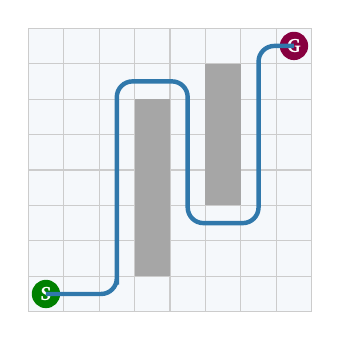
\begin{tikzpicture}[scale=0.45, >=Latex]
      % Grid
      \foreach \x in {0,...,7} {
        \foreach \y in {0,...,7} {
          \fill[fbblau!5] (\x,\y) rectangle (\x+1,\y+1);
          \draw[gray!40] (\x,\y) rectangle (\x+1,\y+1);
        }
      }
      % Obstacles
      \foreach \ox/\oy in {3/1,3/2,3/3,3/4,3/5,5/3,5/4,5/5,5/6} {
        \fill[gray!70] (\ox,\oy) rectangle ++(1,1);
      }
      % Start
      \fill[dkgreen] (0.5,0.5) circle(4mm);
      \node[white, font=\scriptsize\bfseries] at (0.5,0.5) {S};
      % Goal
      \fill[blackberry] (7.5,7.5) circle(4mm);
      \node[white, font=\scriptsize\bfseries] at (7.5,7.5) {G};
      % Path
      \draw[fbblau, ultra thick, rounded corners=2mm]
        (0.5,0.5) -- (2.5,0.5) -- (2.5,0.5)
        -- (2.5,6.5) -- (4.5,6.5)
        -- (4.5,2.5) -- (6.5,2.5)
        -- (6.5,7.5) -- (7.5,7.5);
    \end{tikzpicture}
  \end{column}
\end{columns}

\end{frame}


% -----------------------------------------------------------
\begin{frame}{Trajektorienplanung \& Hindernisvermeidung}

\textbf{Pfad $\neq$ Trajektorie:}
\begin{itemize}
  \item \textbf{Pfad:} geometrische Kurve $(x(s), y(s))$
  \item \textbf{Trajektorie:} Pfad + Zeitparametrisierung
        $(x(t), y(t), \theta(t))$
\end{itemize}

\vspace{2mm}
\textbf{Anforderungen an die Trajektorie:}
\begin{enumerate}
  \item \hl{Glatt:} stetig differenzierbar (keine Sprünge in $v$ oder $\omega$)
  \item \hl{Physikalisch realisierbar:} $v_\mathrm{max}$, $\omega_\mathrm{max}$
        einhalten
  \item \hl{Hindernisfrei:} Sicherheitsabstand zu Objekten
\end{enumerate}

\vspace{3mm}
\textbf{Hindernisvermeidung (reaktiv):}
\begin{itemize}
  \item \textbf{Bug-Algorithmen:} Hindernis umfahren, dann Zielrichtung wieder aufnehmen
  \item \textbf{Potentialfeldmethode:} Ziel = anziehend, Hindernisse = abstoßend
  \item \textbf{Dynamic Window Approach (DWA):} Suche im $(v,\omega)$-Raum
\end{itemize}

\end{frame}


% ============================================================
\section{Softwarearchitektur (ROS\,2)}
% ============================================================

% -----------------------------------------------------------
\begin{frame}{Sensor $\rightarrow$ Topic $\rightarrow$ Node $\rightarrow$ Control Loop}

\begin{center}
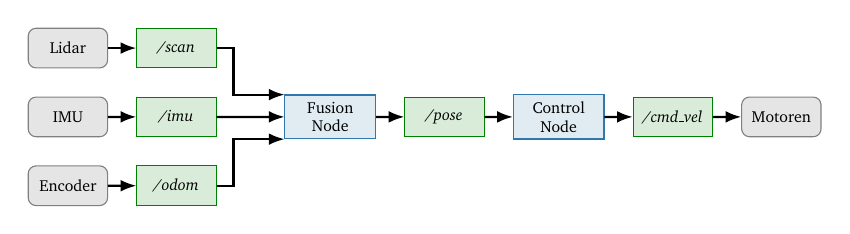
\begin{tikzpicture}[scale=0.72, every node/.style={transform shape},
    node distance=5mm and 5mm,
    hw/.style={rectangle, draw=gray, fill=gray!20,
               minimum width=14mm, minimum height=7mm,
               font=\footnotesize, rounded corners=1mm},
    topic/.style={rectangle, draw=dkgreen, fill=dkgreen!15,
                  minimum width=14mm, minimum height=7mm,
                  font=\footnotesize\itshape},
    nd/.style={rectangle, draw=fbblau, fill=fbblau!15,
               minimum width=16mm, minimum height=7mm,
               font=\footnotesize, align=center},
    arr/.style={-{Latex[length=2mm]}, thick}
  ]
  \node[hw]    (lidar) {Lidar};
  \node[hw, below=of lidar] (imu)   {IMU};
  \node[hw, below=of imu]   (enc)   {Encoder};

  \node[topic, right=of lidar] (tscan) {/scan};
  \node[topic, right=of imu]   (timu)  {/imu};
  \node[topic, right=of enc]   (todom) {/odom};

  \node[nd, right=12mm of timu]  (fuse) {Fusion\\ Node};
  \node[topic, right=of fuse]    (tpose) {/pose};
  \node[nd, right=of tpose]      (ctrl) {Control\\ Node};
  \node[topic, right=of ctrl]    (tcmd) {/cmd\_vel};
  \node[hw, right=of tcmd]       (mot)  {Motoren};

  \draw[arr] (lidar) -- (tscan);
  \draw[arr] (imu)   -- (timu);
  \draw[arr] (enc)   -- (todom);
  % Arrows from topics to fusion node
  \draw[arr] (tscan.east) -- ++(3mm,0) |- (fuse.north west);
  \draw[arr] (timu)  -- (fuse);
  \draw[arr] (todom.east) -- ++(3mm,0) |- (fuse.south west);
  \draw[arr] (fuse)  -- (tpose);
  \draw[arr] (tpose) -- (ctrl);
  \draw[arr] (ctrl)  -- (tcmd);
  \draw[arr] (tcmd)  -- (mot);
\end{tikzpicture}
\end{center}

\vspace{2mm}
\hl{Jede Kante ist ein ROS\,2 Topic} -- lose Kopplung, austauschbare Komponenten.

\end{frame}


% -----------------------------------------------------------
\begin{frame}{ROS\,2 -- Publisher / Subscriber \& QoS}

\begin{columns}[T]
  \begin{column}{0.50\textwidth}
    \textbf{Publisher / Subscriber:}
    \begin{itemize}
      \item Asynchrone Kommunikation
      \item Publisher sendet auf Topic
      \item Subscriber empfängt Callback
      \item Kein direkter Aufruf $\Rightarrow$ Entkopplung
    \end{itemize}

    \vspace{2mm}
    \textbf{Quality of Service (QoS):}
    \begin{itemize}
      \item \texttt{RELIABLE}: jede Nachricht kommt an
            (TCP-ähnlich)
      \item \texttt{BEST\_EFFORT}: keine Garantie
            (UDP-ähnlich, weniger Latenz)
      \item \texttt{KEEP\_LAST(n)}: nur die $n$ neuesten
            Nachrichten puffern
    \end{itemize}
  \end{column}
  \begin{column}{0.45\textwidth}
    \begin{alertblock}{Wichtig für Echtzeit!}
      Falsche QoS-Einstellungen können zu:
      \begin{itemize}
        \item verlorenen Sensordaten
        \item erhöhter Latenz
        \item nicht-deterministischem Verhalten
      \end{itemize}
      führen. $\Rightarrow$ QoS bewusst wählen!
    \end{alertblock}

    \vspace{2mm}
    \textbf{Typische Kombination:}
    \begin{itemize}
      \item Sensordaten: \texttt{BEST\_EFFORT}
      \item Steuerbefehle: \texttt{RELIABLE}
    \end{itemize}
  \end{column}
\end{columns}

\end{frame}


% -----------------------------------------------------------
\begin{frame}[fragile]{Timing: Frequenzen und Latenz}

\begin{columns}[T]
  \begin{column}{0.55\textwidth}
    \textbf{Verschiedene Raten im System:}

    \vspace{1mm}
    \begin{tabular}{lrl}
      \toprule
      \textbf{Komponente} & \textbf{Rate} & \textbf{Typ} \\
      \midrule
      IMU                 & $\SI{200}{Hz}$  & Sensor \\
      Lidar               & $\SI{10}{Hz}$   & Sensor \\
      Kamera              & $\SI{30}{Hz}$   & Sensor \\
      Odometrie           & $\SI{50}{Hz}$   & Verarbeitung \\
      Regelung            & $\SI{20}{Hz}$   & Control \\
      SLAM                & $\SI{1}{Hz}$    & Planung \\
      \bottomrule
    \end{tabular}
  \end{column}
  \begin{column}{0.40\textwidth}
    \textbf{Latenz-Budget:}
    \begin{itemize}
      \item Gesamtlatenz: Sensor $\rightarrow$ Aktor
      \item Muss kleiner als Regelungsperiode sein
      \item Bei $\SI{20}{Hz}$ Control:
            Budget $< \SI{50}{ms}$
    \end{itemize}

    \vspace{2mm}
    \begin{exampleblock}{ROS\,2 Timer}
      \texttt{timer = create\_wall\_timer(}\\
      \texttt{~~50ms, callback);}
    \end{exampleblock}
  \end{column}
\end{columns}

\end{frame}


% ============================================================
\section{Echtzeit und Embedded-Aspekte}
% ============================================================

% -----------------------------------------------------------
\begin{frame}{Sampling Rates vs.\ Control Rates}

\textbf{Kernunterscheidung:}
\begin{itemize}
  \item \hl{Sampling Rate}: Wie oft wird gemessen? (Sensorfrequenz)
  \item \hl{Control Rate}: Wie oft wird geregelt? (Aktorfrequenz)
\end{itemize}

\vspace{3mm}
In der Regel gilt:
$f_\mathrm{sensor} \ge f_\mathrm{control} \ge f_\mathrm{planning}$

\vspace{3mm}
\begin{exampleblock}{Beispiel Turtlebot}
  \begin{tabular}{ll}
    IMU Sampling:        & $\SI{100}{Hz}$ \\
    Encoder Sampling:    & $\SI{50}{Hz}$ \\
    PID Control Loop:    & $\SI{20}{Hz}$ \\
    Pfadplanung:         & $\SI{1}{Hz}$ \\
  \end{tabular}

  \vspace{1mm}
  Jede Schicht konsumiert die Daten der darüberliegenden.
\end{exampleblock}

\end{frame}


% -----------------------------------------------------------
\begin{frame}[fragile]{Determinismus, Interrupts, Polling}

\begin{columns}[T]
  \begin{column}{0.48\textwidth}
    \textbf{Determinismus:}
    \begin{itemize}
      \item Regelschleife muss \warn{garantiert} innerhalb
            der Deadline fertig sein
      \item Linux ist \emph{nicht} echtzeitfähig
            (aber: PREEMPT\_RT Patch)
      \item Microcontroller: oft bare-metal oder RTOS
    \end{itemize}

    \vspace{2mm}
    \textbf{Interrupts vs.\ Polling:}
    \begin{itemize}
      \item \textbf{Interrupt:} Hardware signalisiert Ereignis
            $\Rightarrow$ sofortige Reaktion
      \item \textbf{Polling:} Software fragt zyklisch ab
            $\Rightarrow$ einfacher, aber Latenz
    \end{itemize}
  \end{column}
  \begin{column}{0.48\textwidth}
    \textbf{Hardware-nahe Verarbeitung (C):}
    \begin{itemize}
      \item Direkte Registerzugriffe
      \item Kein dynamisches Speichermanagement
      \item Vorhersagbare Ausführungszeit
    \end{itemize}

    \vspace{2mm}
    \begin{lstlisting}[language=C, basicstyle=\ttfamily\tiny]
// Interrupt Service Routine
void IMU_IRQHandler(void) {
    int16_t raw = IMU->DATA_REG;
    ring_buffer_push(&imu_buf, raw);
    // Keine malloc, printf etc.!
}

// Polling im Main-Loop
while (1) {
    if (timer_elapsed(20ms)) {
        run_pid_controller();
    }
}
    \end{lstlisting}
  \end{column}
\end{columns}

\end{frame}


% ============================================================
\section{Unsicherheit \& Verifikation}
% ============================================================

% -----------------------------------------------------------
\begin{frame}{Umgang mit Unsicherheit}

\textbf{In der Robotik ist \warn{nichts} exakt:}
\begin{itemize}
  \item Sensoren rauschen (Gaussian Noise, Bias)
  \item Modelle sind Approximationen (Radschlupf, Linearisierung)
  \item Die Umgebung ist dynamisch und teilweise unbekannt
\end{itemize}

\vspace{3mm}
\textbf{Konsequenz für den Entwurf:}
\begin{enumerate}
  \item \hl{Probabilistische Modelle:}
        Zustand als Wahrscheinlichkeitsverteilung, nicht als Punkt
  \item \hl{Robuste Regelung:}
        Sicherheitsmargen in Geschwindigkeit und Abstand
  \item \hl{Defensive Planung:}
        Worst-Case-Szenarien einplanen
\end{enumerate}

\vspace{3mm}
\begin{block}{Safety-Anforderung (Beispiel)}
  ``Der Roboter hält \emph{immer} mindestens $\SI{30}{cm}$
  Abstand zu jedem Hindernis'' -- unabhängig von Sensorrauschen.
\end{block}

\end{frame}


% -----------------------------------------------------------
\begin{frame}{Formale Verifikation: Timed Automata}

\textbf{Rückgriff auf die Modellierungstechniken der Vorlesung!}

\vspace{2mm}
\begin{columns}[T]
  \begin{column}{0.50\textwidth}
    \textbf{Timed Automata für Control Loops:}
    \begin{itemize}
      \item Zustände: \texttt{Idle}, \texttt{Sensing},
            \texttt{Computing}, \texttt{Actuating}
      \item Uhren: $c_\mathrm{sense}$, $c_\mathrm{ctrl}$
      \item Guards: $c_\mathrm{ctrl} \le \SI{50}{ms}$
      \item Invarianten erzwingen Deadlines
    \end{itemize}

    \vspace{2mm}
    \textbf{Safety-Eigenschaften:}
    \begin{itemize}
      \item ``Control-Schleife terminiert immer
            innerhalb von $\SI{50}{ms}$''
      \item ``Sensordaten sind nie älter als $\SI{100}{ms}$''
    \end{itemize}
  \end{column}
  \begin{column}{0.45\textwidth}
    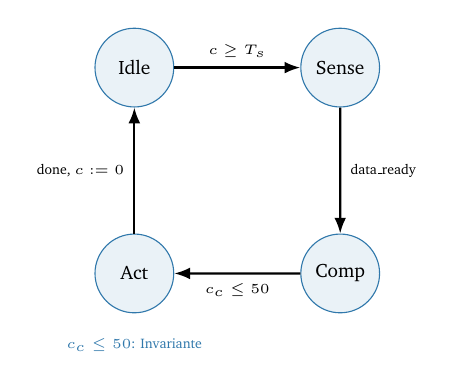
\begin{tikzpicture}[
        scale=0.75,
        node distance=16mm,
        state/.style={circle, draw=fbblau, fill=fbblau!10,
                      minimum size=10mm, font=\scriptsize},
        arr/.style={-{Latex[length=2mm]}, thick}
      ]
      \node[state] (idle)    {Idle};
      \node[state, right=of idle] (sense)  {Sense};
      \node[state, below=of sense] (comp)   {Comp};
      \node[state, below=of idle]  (act)    {Act};

      \draw[arr] (idle)  -- (sense)
        node[midway, above, font=\tiny]{$c \ge T_s$};
      \draw[arr] (sense) -- (comp)
        node[midway, right, font=\tiny]{data\_ready};
      \draw[arr] (comp)  -- (act)
        node[midway, below, font=\tiny]{$c_c \le 50$};
      \draw[arr] (act)   -- (idle)
        node[midway, left, font=\tiny]{done, $c := 0$};

      \node[font=\tiny, fbblau, below=2mm of act]
        {$c_c \le 50$: Invariante};
    \end{tikzpicture}
  \end{column}
\end{columns}

\end{frame}


% -----------------------------------------------------------
\begin{frame}{Verifikation mit UPPAAL}

\textbf{UPPAAL} (bekannt aus der Vorlesung) eignet sich hervorragend
für die Verifikation von Robotik-Scheduling:

\vspace{3mm}
\begin{columns}[T]
  \begin{column}{0.55\textwidth}
    \textbf{Modellierung:}
    \begin{itemize}
      \item Jede Task (Sensor, Filter, Control) als
            Timed Automaton
      \item Kommunikation über Channels
      \item Shared Variables für Sensordaten
    \end{itemize}

    \vspace{2mm}
    \textbf{Verifikation (CTL):}
    \begin{itemize}
      \item \texttt{A[] not deadlock}\\
            {\scriptsize (kein Deadlock möglich)}
      \item \texttt{A[] ctrl.active imply c\_ctrl <= 50}\\
            {\scriptsize (Deadline wird immer eingehalten)}
      \item \texttt{A[] distance >= 30}\\
            {\scriptsize (Sicherheitsabstand garantiert)}
    \end{itemize}
  \end{column}
  \begin{column}{0.40\textwidth}
    \begin{alertblock}{Bezug zur Vorlesung}
      \begin{itemize}
        \item FSMs $\rightarrow$ Verhalten
        \item Timed Automata $\rightarrow$ Timing
        \item UPPAAL $\rightarrow$ Verifikation
        \item C / Rust $\rightarrow$ Implementierung
        \item ROS\,2 $\rightarrow$ Integration
      \end{itemize}
      Alle Werkzeuge kommen hier zusammen!
    \end{alertblock}
  \end{column}
\end{columns}

\end{frame}


% -----------------------------------------------------------
\begin{frame}{Wie verifiziert man probabilistische Systeme?}

\textbf{Problem:} Kalman, SLAM, RL -- alle arbeiten mit \hl{Wahrscheinlichkeiten}.
Klassische Model Checker (UPPAAL) prüfen nur ja/nein-Eigenschaften.

\vspace{2mm}
\begin{columns}[T]
  \begin{column}{0.48\textwidth}
    \textbf{Probabilistic Model Checking:}
    \begin{itemize}\setlength{\itemsep}{1pt}
      \item Modelle: \textbf{DTMC}, \textbf{MDP}, \textbf{CTMC}
            (Markov-Ketten mit/ohne Nichtdeterminismus)
      \item Spezifikation: \textbf{PCTL} / \textbf{CSL}\\
            z.\,B. $\mathcal{P}_{\geq 0.99}[\lozenge\;\textit{goal}]$\\
            {\scriptsize „Ziel wird mit $\geq 99\%$ erreicht"}
      \item $\mathcal{P}_{\leq 10^{-6}}[\lozenge\;\textit{collision}]$\\
            {\scriptsize „Kollision mit $\leq 0.0001\%$"}
    \end{itemize}
  \end{column}
  \begin{column}{0.48\textwidth}
    \textbf{Werkzeuge:}
    \begin{itemize}\setlength{\itemsep}{1pt}
      \item \textbf{PRISM} -- probabilistischer Model Checker
      \item \textbf{Storm} -- effizient für große Modelle
      \item \textbf{UPPAAL SMC} -- Statistical Model Checking
            (Monte-Carlo statt exakt)
    \end{itemize}

    \vspace{2mm}
    \textbf{Brücke zu UPPAAL:}\\
    UPPAAL SMC kann \emph{stochastische}
    Timed Automata simulieren und
    probabilistische Queries beantworten.
  \end{column}
\end{columns}

\vspace{1mm}
\begin{exampleblock}{Robotik-Anwendung}
  \vspace{-2mm}
  Sensorrauschen als stochastisches Modell $\rightarrow$ „Wie wahrscheinlich ist Kollision bei Sensorausfall?" formal prüfbar.\vspace{-2mm}
\end{exampleblock}

\end{frame}


% ============================================================
\section{Zusammenfassung}
% ============================================================

% -----------------------------------------------------------
\begin{frame}{Zusammenfassung: Von Sensoren zur sicheren Robotik}

\begin{center}
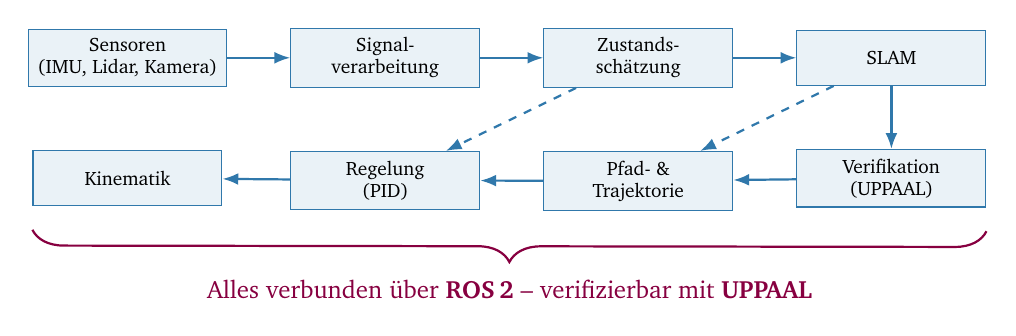
\begin{tikzpicture}[
    node distance=5mm and 8mm,
    box/.style={rectangle, draw=fbblau, fill=fbblau!10,
                minimum width=24mm, minimum height=7mm,
                text centered, font=\scriptsize, align=center},
    arr/.style={-{Latex[length=2mm]}, thick, fbblau}
  ]
  \node[box] (sens)  {Sensoren\\ (IMU, Lidar, Kamera)};
  \node[box, right=of sens]  (sig)   {Signal-\\ verarbeitung};
  \node[box, right=of sig]   (state) {Zustands-\\ sch\"atzung};
  \node[box, right=of state] (slam)  {SLAM};
  \node[box, below=8mm of sens]  (kin)   {Kinematik};
  \node[box, below=8mm of sig]   (ctrl)  {Regelung\\ (PID)};
  \node[box, below=8mm of state] (plan)  {Pfad- \&\\ Trajektorie};
  \node[box, below=8mm of slam]  (verif) {Verifikation\\ (UPPAAL)};

  \draw[arr] (sens) -- (sig);
  \draw[arr] (sig) -- (state);
  \draw[arr] (state) -- (slam);
  \draw[arr] (slam) -- (verif);
  \draw[arr] (plan) -- (ctrl);
  \draw[arr] (ctrl) -- (kin);
  \draw[arr] (verif) -- (plan);

  % Vertical connections
  \draw[arr, dashed] (state) -- (ctrl);
  \draw[arr, dashed] (slam) -- (plan);

  % ROS 2 bracket -- anchored below the lower row of nodes
  \draw[decorate, decoration={brace, amplitude=4mm, mirror},
        blackberry, thick]
    ([yshift=-3mm]kin.south west) -- ([yshift=-3mm]verif.south east)
    node[midway, below=5mm, font=\small, blackberry]
    {Alles verbunden \"uber \textbf{ROS\,2} -- verifizierbar mit \textbf{UPPAAL}};
\end{tikzpicture}
\end{center}

\end{frame}


% -----------------------------------------------------------
\begin{frame}{Kernbotschaften}

\begin{enumerate}
  \item \textbf{Sensoren sind ungenau} -- Rauschen, Bias und Drift
        müssen modelliert und gefiltert werden.
  \item \textbf{Kalman-Filter} ist das zentrale Werkzeug für
        Zustandsschätzung unter Unsicherheit.
  \item \textbf{Kinematik} verbindet Steuergrößen mit Bewegung --
        Forward und Inverse Kinematics.
  \item \textbf{PID-Regelung} ist der Arbeitspferd-Regler;
        Stabilität muss beachtet werden.
  \item \textbf{SLAM} löst das Henne-Ei-Problem der gleichzeitigen
        Lokalisierung und Kartierung.
  \item \textbf{Echtzeit} ist kein Nice-to-have: Deadlines müssen
        eingehalten werden.
  \item \textbf{Formale Verifikation} (Timed Automata, UPPAAL)
        schließt den Kreis zur sicheren Implementierung.
\end{enumerate}

\end{frame}


% -----------------------------------------------------------
\begin{frame}{Durchgehendes Beispiel: Ein Turtlebot-Zyklus}

\textbf{Szenario:} Turtlebot soll von $(0,0)$ zum Ziel $(3,2)$ fahren.

\vspace{2mm}
\begin{center}
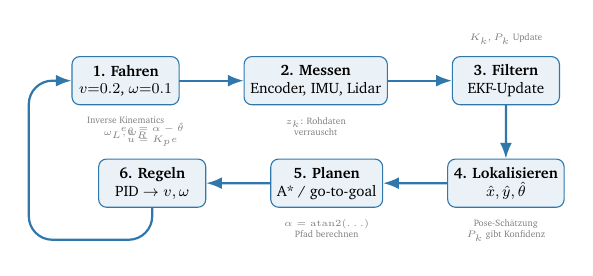
\begin{tikzpicture}[scale=0.68, every node/.style={transform shape},
    node distance=3mm and 6mm,
    stp/.style={rectangle, draw=fbblau, fill=fbblau!10,
                minimum width=20mm, minimum height=9mm,
                text centered, font=\footnotesize, align=center,
                rounded corners=1mm},
    data/.style={font=\tiny, text=gray, align=center},
    arr/.style={-{Latex[length=2mm]}, thick, fbblau}
  ]
  \node[stp] (drive) {\textbf{1. Fahren}\\ $v{=}0.2$, $\omega{=}0.1$};
  \node[stp, right=12mm of drive] (sense) {\textbf{2. Messen}\\ Encoder, IMU, Lidar};
  \node[stp, right=12mm of sense] (filt) {\textbf{3. Filtern}\\ EKF-Update};
  \node[stp, below=10mm of filt] (loc) {\textbf{4. Lokalisieren}\\ $\hat{x},\hat{y},\hat{\theta}$};
  \node[stp, left=12mm of loc] (plan) {\textbf{5. Planen}\\ A* / go-to-goal};
  \node[stp, left=12mm of plan] (ctrl) {\textbf{6. Regeln}\\ PID $\to v,\omega$};

  \draw[arr] (drive) -- (sense);
  \draw[arr] (sense) -- (filt);
  \draw[arr] (filt) -- (loc);
  \draw[arr] (loc) -- (plan);
  \draw[arr] (plan) -- (ctrl);
  \draw[arr, rounded corners=3mm] (ctrl.south) -- ++(0,-6mm) -| ([xshift=-8mm]drive.west) -- (drive.west);

  % Annotations
  \node[data, below=1mm of drive] {Inverse Kinematics\\$\omega_L, \omega_R$};
  \node[data, below=1mm of sense] {$z_k$: Rohdaten\\verrauscht};
  \node[data, above=1mm of filt] {$K_k$, $P_k$ Update};
  \node[data, below=1mm of loc] {Pose-Schätzung\\$P_k$ gibt Konfidenz};
  \node[data, below=1mm of plan] {$\alpha = \mathrm{atan2}(\ldots)$\\Pfad berechnen};
  \node[data, above=1mm of ctrl] {$e_\theta = \alpha - \hat{\theta}$\\$u = K_p e$};
\end{tikzpicture}
\end{center}

Jede Runde dauert $\Delta t = \SI{50}{ms}$ ($\SI{20}{Hz}$).
Der Zyklus wiederholt sich, bis $\|\hat{\mathbf{p}} - \mathbf{p}_\mathrm{goal}\| < \epsilon$.

\end{frame}


% -----------------------------------------------------------
\begin{frame}{Turtlebot-Zyklus -- Zahlenbeispiel}

\textbf{Zeitschritt $k=42$:} Roboter bei $\hat{x} \approx 1.8$, $\hat{y} \approx 1.1$, $\hat{\theta} \approx 0.5\,\text{rad}$

\vspace{2mm}
\begin{enumerate}
  \item \textbf{Messen:}
        Encoder: $v_\mathrm{enc} = 0.19\,\text{m/s}$ \;
        IMU: $\omega_\mathrm{imu} = 0.12\,\text{rad/s}$ \;
        Lidar: $(x_L, y_L) = (1.83, 1.08)$

  \item \textbf{EKF-Prädiktion} ($\Delta t = 0.05\,\text{s}$):
        \begin{align*}
          \hat{x}^- &= 1.8 + 0.2 \cdot \cos(0.5) \cdot 0.05 = 1.8088 \\[-1mm]
          \hat{y}^- &= 1.1 + 0.2 \cdot \sin(0.5) \cdot 0.05 = 1.1048 \\[-1mm]
          \hat{\theta}^- &= 0.5 + 0.1 \cdot 0.05 = 0.505
        \end{align*}

  \item \textbf{EKF-Update} (Lidar-Korrektur):
        Innovation $(1.83 - 1.8088,\; 1.08 - 1.1048) = (0.021, -0.025)$ \\
        $\Rightarrow$ Kalman-Gain korrigiert Pose leicht Richtung Lidar.

  \item \textbf{Planen:} Richtung zum Ziel
        $\alpha = \mathrm{atan2}(2 - 1.10,\; 3 - 1.81) \approx 0.645\,\text{rad}$

  \item \textbf{Regeln:}
        $e_\theta = 0.645 - 0.505 = 0.14$ \;$\Rightarrow$\;
        $\omega = K_p \cdot 0.14 = 0.28\,\text{rad/s}$
\end{enumerate}

$\Rightarrow$ Nächster Schritt: etwas mehr nach links lenken, weiterfahren.

\end{frame}


% ============================================================
\section*{Exkurs: Reinforcement Learning}
% ============================================================

% -----------------------------------------------------------
\begin{frame}{Exkurs: Reinforcement Learning (RL)}

\textbf{Bisher:} Modellbasierte Ansätze -- wir kennen das
physikalische Modell und entwerfen Regler analytisch (PID, Kalman).

\vspace{2mm}
\textbf{Alternative:} Was wenn das Modell zu komplex oder unbekannt ist?

\vspace{2mm}
\begin{block}{Reinforcement Learning}
  Ein \hl{Agent} lernt durch \hl{Trial-and-Error}, welche
  \hl{Aktion} $a$ in welchem \hl{Zustand} $s$ die höchste
  \hl{kumulative Belohnung} $R$ liefert.
\end{block}

\vspace{2mm}
\begin{center}
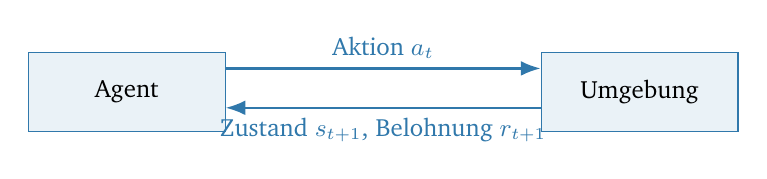
\begin{tikzpicture}[
    node distance=10mm and 25mm,
    box/.style={rectangle, draw=fbblau, fill=fbblau!10,
                minimum width=25mm, minimum height=10mm,
                text centered, font=\small},
    arr/.style={-{Latex[length=2.5mm]}, thick, fbblau}
  ]
  \node[box] (agent) {Agent};
  \node[box, right=40mm of agent] (env) {Umgebung};

  \draw[arr] ([yshift=3mm]agent.east) -- ([yshift=3mm]env.west)
    node[midway, above, font=\small]{Aktion $a_t$};
  \draw[arr] ([yshift=-2mm]env.west) -- ([yshift=-2mm]agent.east)
    node[midway, below, font=\small]{Zustand $s_{t+1}$, Belohnung $r_{t+1}$};
\end{tikzpicture}
\end{center}

\vspace{1mm}
Formal: Markov Decision Process (MDP)
$(S, A, P, R, \gamma)$.

\end{frame}


% -----------------------------------------------------------
\begin{frame}{RL -- Grundbegriffe}

\textbf{Ziel:} Finde eine \hl{Policy} $\pi(a|s)$, die den erwarteten
diskontierten Gesamtnutzen maximiert:
\[
  J(\pi) = \mathrm{E}_\pi\!\left[\sum_{t=0}^{\infty} \gamma^t\, r_{t+1}\right]
\]
mit Diskontfaktor $\gamma \in [0,1)$.

\vspace{3mm}
\textbf{Kernkonzepte:}
\begin{itemize}
  \item \textbf{Value-Funktion} $V^\pi(s)$: erwarteter Gesamtnutzen ab Zustand $s$
        \[
          V^\pi(s) = \mathrm{E}_\pi\!\left[\sum_{t=0}^\infty \gamma^t r_{t+1} \;\middle|\; s_0 = s\right]
        \]
  \item \textbf{Q-Funktion} $Q^\pi(s,a)$: wie $V$, aber zusätzlich bedingt auf Aktion $a$
  \item \textbf{Bellman-Gleichung:}
        $Q^\pi(s,a) = r(s,a) + \gamma \sum_{s'} P(s'|s,a)\,V^\pi(s')$
  \item \textbf{Exploration vs.\ Exploitation:}
        Neues ausprobieren vs.\ bekannte gute Strategien nutzen
\end{itemize}

\end{frame}


% -----------------------------------------------------------
\begin{frame}{RL-Algorithmen -- Überblick}

\begin{columns}[T]
  \begin{column}{0.48\textwidth}
    \textbf{Tabellarische Methoden:}
    \begin{itemize}
      \item \textbf{Q-Learning:}\\
            Lerne $Q(s,a)$-Tabelle iterativ
      \item Update:
            {\small $Q(s,a) \leftarrow Q(s,a) + \alpha\,[r + \gamma \max_{a'} Q(s',a') - Q(s,a)]$}
      \item Konvergiert zum Optimum
      \item Nur für \warn{kleine, diskrete}
            Zustands-/Aktionsräume
    \end{itemize}
  \end{column}
  \begin{column}{0.48\textwidth}
    \textbf{Für Robotik:}
    \begin{itemize}
      \item Zustandsraum ist \emph{kontinuierlich}
            $(x, y, \theta, v, \omega, \ldots)$
      \item Aktionsraum ist \emph{kontinuierlich}
            $(v_\mathrm{cmd}, \omega_\mathrm{cmd})$
      \item Q-Tabelle unmöglich
            (unendlich viele Einträge)
      \item $\Rightarrow$ Funktionsapproximation nötig
    \end{itemize}
  \end{column}
\end{columns}

\vspace{4mm}
\begin{alertblock}{Motivation für Deep RL}
  Neuronale Netze als universelle Funktionsapproximatoren
  können $Q(s,a)$ oder $\pi(a|s)$ für kontinuierliche Räume lernen.
\end{alertblock}

\end{frame}


% -----------------------------------------------------------
\begin{frame}{Deep Reinforcement Learning}

\textbf{Idee:} Ersetze die Q-Tabelle / Policy durch ein
\hl{neuronales Netz} mit Parametern $\theta$.

\vspace{3mm}
\begin{columns}[T]
  \begin{column}{0.48\textwidth}
    \textbf{Value-based (DQN):}
    \begin{itemize}
      \item Netz approximiert $Q_\theta(s,a)$
      \item Trainiert mit Experience Replay
      \item Funktioniert für diskrete Aktionen
      \item Durchbruch: Atari-Spiele (2015)
    \end{itemize}

    \vspace{2mm}
    \textbf{Policy-based:}
    \begin{itemize}
      \item Netz gibt direkt $\pi_\theta(a|s)$ aus
      \item Gradient: $\nabla_\theta J \approx$\\
            $\mathrm{E}[\nabla_\theta \log\pi_\theta \cdot R]$
      \item Funktioniert für \hl{kontinuierliche} Aktionen
    \end{itemize}
  \end{column}
  \begin{column}{0.48\textwidth}
    \textbf{Actor-Critic (z.\,B.\ PPO, SAC):}
    \begin{itemize}
      \item \textbf{Actor:} Policy-Netz $\pi_\theta(a|s)$
      \item \textbf{Critic:} Value-Netz $V_\phi(s)$
      \item Critic bewertet die Aktionen des Actors
      \item Stabiler als reines Policy Gradient
    \end{itemize}

    \vspace{2mm}
    \textbf{Für Robotik besonders relevant:}
    \begin{itemize}
      \item \textbf{PPO} (Proximal Policy Optimization)
      \item \textbf{SAC} (Soft Actor-Critic)
      \item \textbf{TD3} (Twin Delayed DDPG)
    \end{itemize}
  \end{column}
\end{columns}

\end{frame}


% -----------------------------------------------------------
\begin{frame}{Deep RL in der Robotik -- Chancen und Grenzen}

\begin{columns}[T]
  \begin{column}{0.48\textwidth}
    \textbf{Wo Deep RL gut funktioniert:}
    \begin{itemize}
      \item Laufroboter (Locomotion)
      \item Greifplanung (Manipulation)
      \item Hindernisvermeidung in\\
            unbekannter Umgebung
      \item Wenn physikalisches Modell\\
            zu komplex oder unbekannt
    \end{itemize}

    \vspace{2mm}
    \textbf{Sim-to-Real:}\\
    Training in Simulation, Transfer auf realen Roboter.
    Spart Millionen von Episoden auf realer Hardware.
  \end{column}
  \begin{column}{0.48\textwidth}
    \textbf{Offene Herausforderungen:}
    \begin{itemize}
      \item \warn{Sample Inefficiency:}
            Millionen Episoden für Training
      \item \warn{Safety:}
            Wie verhindert man gefährliches Verhalten während des Lernens?
      \item \warn{Interpretierbarkeit:}
            Neuronales Netz ist Black Box
      \item \warn{Sim-to-Real Gap:}
            Simulation $\neq$ Realität
    \end{itemize}
  \end{column}
\end{columns}

\vspace{1mm}
\begin{block}{Abgrenzung zu modellbasierten Methoden}
  \vspace{-1mm}
  PID + Kalman + SLAM: \textbf{interpretierbar, verifizierbar, deterministisch}.
  Deep RL: \textbf{flexibel, lernfähig, aber schwer zu verifizieren}.
  Praxis: modellbasiert + RL für Feintuning.\vspace{-1mm}
\end{block}

\end{frame}


% ============================================================
\end{document}
% ============================================================
